\documentclass{article}
\usepackage[utf8]{inputenc}
\usepackage[T1]{fontenc}
\usepackage{subcaption}
\usepackage{float}
\usepackage{amsmath,amssymb}
\usepackage{mathabx}
\usepackage{adjustbox}
\title{Unsupervised Domain Adaptation with Gradient Reversal Layer and its modifications}
\author{Wojciech Pratkowiecki}

\usepackage[utf8]{inputenc}
\usepackage[english]{babel}
\usepackage[
backend=biber,
style=numeric,
sorting=none
]{biblatex}
\addbibresource{main_bibliography.bib}
\usepackage{graphicx}

\begin{document}

\maketitle

\begin{abstract}
The amount of data that is still unlabeled has been growing over recent years. With domain adaptation methods it is possible to get a model that classifies well these samples, if only a related and labeled set is available. Therefore, the popularity of domain adaptation has strongly increased. While trying to get better and better results, many diverse and complex approaches were invented. This paper describes research and experiments aimed at understanding the problem of domain adaptation and coping with it using the Gradient Reversal Layer.
\end{abstract}

\section{Introduction}
Neural networks have found many applications in recent years due to their ability of learning some complex data dependencies. Top performance in various tasks have resulted in increased popularity of not only neural networks and deep learning but also of other machine learning (ML) methods. Different architectures designed for different tasks were invented. One of them is convolutional neural network (CNN) introduced by Yann LeCun \cite{cnn}, which caused huge improvement in the image classification field. However, obtaining top-performing models often requires a long training, with huge amount of labeled data. Such a complicated procedure yields a desired model, but it would not reach comparable results on different, even strongly related dataset. Moreover, if we  have small amount of labeled samples, we need to find an alternative way to train the network. At this point domain adaptation is an attractive option.
\par
Domain adaptation (DA) is a process of learning a distribution of samples from source domain and obtain a model that performs well on other, but related, target domain. For instance, if we have a huge (e.g. synthetic), labeled set of road signs images and a video from a ride through a city, we could get an effective model that classifies well all the signs from the video frames, if we train it properly with the labeled dataset. One of domain adaptation techniques is the Gradient Reversal Layer (GRL) proposed by Yaroslav Ganin and Victor Lempitsky \cite{pmlr-v37-ganin15}. GRL is a simple, but effective, architectural trick, applied during backpropagation, designed especially for domain adaptation task. This thesis is a collection of research on the Gradient Reversal Layer and its adjustments. I tried not only to improve the results but also to get a detailed understanding of domain adaptation problem and GRL behaviour.

\section{Background knowledge}
\subsection{Artificial neural network}

Artificial neural network (ANN) is a machine learning technique inspired by neural connections in human brain. While training the model we use a pre-defined architecture and loss function. The architecture describes the transformation of the input data made by our model, its complexity and interpretation of the output. Each network contains neurons that are stacked in layers. Neurons are nothing but a weighted sum characterized by neuron's weights and bias. A layer is built with many neurons and followed by non-linear activation function. Each layer transforms its input vector into an output vector. The first layer of the network is called the input layer, the last one is the output layer, while all the intermediate layers are called hidden layers. Figure~\ref{fig:ANN} presents a sample ANN. The loss function is a way to measure and optimize the performance of the model, it is commonly the magnitude of its imprecision.
\par
Successful learning process requires many examples of the problem we want the network to solve. At the beginning, we usually set the model's parameters (mostly denoted as $\Theta$) to random values. The model transforms some of the input examples and we compute the loss function based on the output. As we want the model to perform as well as possible, our goal is to minimize the loss function. Therefore we use the backpropagation method - for each input sample we compute its gradient. The values of those gradients tell us, how should we tune model's parameters $\Theta$ to find the minimum of loss function. Therefore, we slightly change values of $\Theta$ in the direction of gradient, which should recall in a better performance of the model on the next examples. We repeat this process many times, improving our network during whole learning process. 
\par
This iterative training approach is a simplified description of stochastic gradient descent (SGD) - one of the most popular and effective ANN optimization method. As our model may be defined by millions of parameters, computational cost of thousands of training iterations is a huge drawback of neural networks. However, great growth of computer's computation power with GPU acceleration let us find solutions for some really complex problems within decent time.  Therefore neural networks are nowadays widely used for many tasks. One of them is image classification - finding for a given input image the most likely label from a fixed label set.

\subsection{Convolutional neural networks}
Applying neural networks to image processing became very popular. To keep reaching better results in tasks like image classification some new inventions were needed. The breakthrough came with convolutional neural networks (CNN). CNN, just like classical neural network, is built with neurons stacked in layers. First layers of CNN are convolution layers. Each of them is a set of learnable, small size (like 5$\times$5) filters followed by activation function. Each filter processes input image step by step and produces a transformed, usually smaller, one. Therefore after each layer we get a new set of images obtained from all pictures from previous layer. A big advantage of this approach is a much smaller number of learnable parameters - if the input image has size 1000 $\times$ 1000 it would require 1000000 parameters for a single neuron in a fully connected layer, while convolution layer processes it with its filter, that has 25 parameters, if the size of the filter is 5$\times$5.  After a convolution layer we usually use pooling - we divide the picture into cells (e.g. of size 2$\times$2) and we replace the whole cell with its maximum value (in case of maximum pooling). This operation reduces the size of the image internal representation, and force the network to focus on important patterns. Figure~\ref{fig:CNN} presents an example of CNN architecture.
\par
The convolutional part of the model learns high-level features or descriptors of locations in the input image. Moreover it makes the network invariant for small translation of object over the image. If our model classifies dog breeds, it will give the same result, no matter if the dog is in the middle or in a corner of the photo. Convolutional layers produce a vector representation of the input image. It is then fed into classical, fully-connected layers that return the model's output. If our task is image classification the output is a vector of classes probabilities typically.
\par
CNNs caused huge improvements in both accuracy and speed of image classification. Nowadays top-performing architectures in many image processing problems are built with convolutions. Convolutional layers also found application in some non-picture field like some natural language processing tasks or speech generation. 

\begin{figure}[htb]%
    \centering
    \includegraphics[width=\linewidth]{ANN.jpeg}%
    \caption{Example of neural network architecture. Picture from Staford course website \cite{stanford}}%
    \label{fig:ANN}%
\end{figure}
\begin{figure}[htb]%
    \centering
    \includegraphics[width=\linewidth]{CNN.png}%
    \caption{Example of convolutional neural network architecture. Picture from \cite{cnn_im}}%
    \label{fig:CNN}%
\end{figure}

\subsection{Digit classification with CNN}
MNIST dataset \cite{mnist} is a collection of black and white photos of handwritten digits. Every picture's resolution is 28$\times$28 pixels, each one is an integer in the range $[0,255]$, that describes the brightness of the pixel. All the samples are provided with ground truth labels. Classification of digit images is therefore a task of processing the input image that dimensionality is 28$\times$28, and assigning probabilities for each of 0-9 digits. The model prediction is the digit with highest probability. Even very ordinary convolutional architecture reaches over 99\% accuracy on this dataset. A bit more challenging modification of MNIST is the MNIST-M set \cite{mnist-m}, obtained by blending example from MNIST with some color photos from BSDS500. There is probably no difference in difficulty of classification MNIST and MNIST-M digits for human, but from neural network point of view, the colorful set is much more complex. Nevertheless, obtaining top-performing model is relatively easy.
\par
There are a lot of similar digit recognition datasets, with many that are much more complex than MNIST and its modifications. The Street View House Number (SVHN) is a good example of such collection. SVHN samples are obtained from Google Street View photos, therefore they are colorful, with diverse backgrounds, pictures are often blurry and a single image may present few digits, while its label is the one in the centre of the photo. Due to all those properties of SVHN, model that classifies well its samples must be complex and longer trained. 
\par
Even though digit classification seems not to be the most important and entertaining problem that CNN may solve, it is still one of the most popular field of measuring a model's performance and yields experimental results with quick turn-around time. Figure~\ref{fig:digits} presents some examples from mentioned datasets - MNIST, MNIST-M and SVHN.

\begin{figure}%
    \centering
    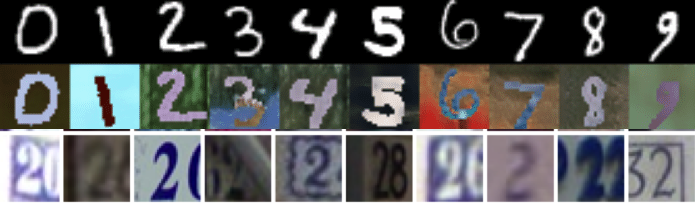
\includegraphics[width=\linewidth]{digits.png}%
    \caption{Samples from MNIST, MNIST-M and SVHN digit images datasets, best viewed in color}
    \label{fig:digits}%
\end{figure}

\subsection{Domain adaptation}
Let's suppose that we have a novel, large set of digit images, for instance photos of the back of each European footballer's jersey, preprocessed in a way, that every image contains one digit - figure~\ref{fig:football} presents some possible samples. Our goal is to obtain a model that classifies digits from football kits. Unfortunately we don't have any labels for these pictures, so we are unable to go a straightforward way and train a CNN adjusted to the image set, as we cannot determinate if the model's prediction is right. In this kind of situation domain adaptation is a solution.
\par
Domain adaptation is a specific training process, when we teach a model with examples from a source domain, but our goal is to make it perform well on different, but related, target domain. Over recent years many architectures have been proposed to reach as high target domain accuracy as possible. DA is needed when samples from target distribution are unlabeled (unsupervised domain adaptation) or we have just few labeled examples (semi-supervised domain adaptation). A model should find a mapping between domains, which would allow source domain classifier perform well on test (target domain) examples.
\par
In our case of football jerseys, when the set is unlabeled at all, we have an unsupervised DA problem. Target domain is the distribution of jersey's photos. Now we should try to obtain a model learned with labeled examples from other dataset, like SVHN, and apply some architectural solution that would let the model classify well digits from football kits. Dozens of such tricks have been proposed in recent years. One of them is Gradient Reversal Layer.

\begin{figure}%
    \centering
    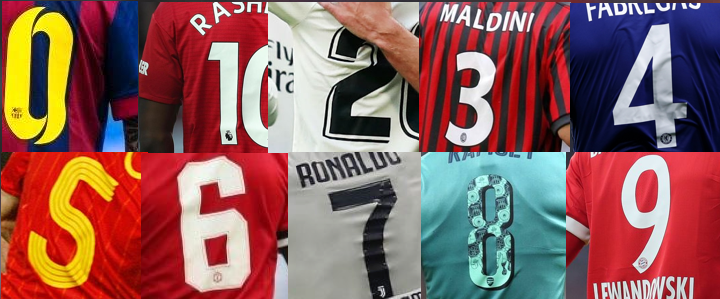
\includegraphics[width=\linewidth]{football.png}%
    \caption{Football jersey dataset}
    \label{fig:football}%
\end{figure}


\subsection{Gradient reversal layer}
Gradient Reversal Layer was introduced by Yaroslav Ganin and Victor Lempitsky in the paper titled "Unsupervised Domain Adaptation by Backpropagation" in 2015 \cite{pmlr-v37-ganin15}. The authors describe domain adaptation as a problem of finding common mapping for source and target distribution, that would transform samples to some kind of representation that allows classifier perform well and does not contain any information about the domain of mapped sample. In perfect scenario the mapping does not influence the label predictor's accuracy, but is so invariant w.r.t. domain shift that we cannot obtain a model, that predicts well the distribution of the input.
\par
Gradinet Reversal Layer itself is a simple trick used during backpropagation pass. It is a trival layer in network's architecture, that leaves the input unchanged during forward propagation, but multiplies the gradinet by negative scalar $\lambda$ during backpropagation. Formally we could say that GRL is a function specified as:
\begin{equation*}
GRL(x, \lambda) = \begin{cases}
x &\text{forward pass}\\
-\lambda \cdot x &\text{backward pass}
\end{cases}
\end{equation*}
GRL demands a special architecture, contructed with three parts - a \textit{feature extractor}, that is denoted as $G_{f}$ and maps the input to a $D$-dimensional vector $f \in \mathbb{R}^{D}$. Feature extractor is a neural network with its parameters $\Theta_{f}$, so the transformation of input vector $x$ is denoted as $G_{f}(x;\Theta_{f})$. This representation is then used by two other components of the model - a \textit{class predictor} $G_{y}$ with parameters $\Theta_{y}$, that classifies the $f = G_{f}(x;\Theta_{f})$ vector, 
and a \textit{domain predictor} $G_{d}$ with its parameters denoted as $\Theta_{d}$, which task is to predict the domain label of the vector $f$. The very first layer of $G_{d}$ is the GRL, therefore during backpropagation the gradient that comes to the feature extractor from domain predictor is multiplied by -$\lambda$. Figure~\ref{fig:GRLarch} presents a diagram with described architecture.
\par
All those three components are independent neural networks that construct our architecture. While training the model we aim to force $G_{f}$ to yield domain-invariant feature vectors $f$. GRL placed at the beginning of $G_{d}$ should be very helpful. The intuition behind inversion of the gradient sign during backpropagation is to follow the opposite direction to the domain predictor gradient, so after each update of the parameters of feature extractor, the feature vector $f$ should be more involved for $G_{d}$ and a good prediction of its domain label - much harder. $G_{d}$ itself tries to minimize its own loss function to make better predictions. If the domain predictor, that wants to does its best, is unable to determinate the distribution of the $f$, then $f$ is getting more domain-invariant. In perfect scenario GRL has such an impact on $\Theta_{f}$, that $G_{d}$ has the same accuracy as random model. Concurrently $G_{y}$ tries to predict a class of each sample and we try to minimize its loss function. Class predictor's gradient is used to tune $\Theta_{y}$ and then passed do feature extractor. Therefore the feature extractor's parameters are tuned w.r.t. gradient of $G_{y}$ and a negatively multiplied gradient of $G_{d}$. If we denote loss for class prediction as $L_{y}$ and loss for domain classification as $L_{d}$ then our goal is to minimize the function:
\begin{align*} 
E(\Theta_{f}, \Theta_{y}, \Theta_{d}) = &\sum_{\substack{i=1.N \\ d_{i}=0}} L_{y}(G_{y} (G_{f}(x_{i};\Theta_{f}); \Theta_{y} ), y_{i} ) - \\
 &\lambda \cdot \sum_{\substack{i=1.N \\ d_{i}=0,1}} L_{d}(G_{d} (G_{f}(x_{i};\Theta_{f}); \Theta_{d} ), d_{i} )
\end{align*}
where $(x_{i}, y_{i})$ are samples from $d_{i}$ and values $i$ of $d_{i}$ are 0 for source domain and 1 for target domain. Label predictor $G_{y}$ does not classify samples from target domain (as we don't have labels for them), so during the training this part of architecture doesn't even see any example from target distribution. Domain predictor of course process samples from both source and target distribution. The $\lambda$ coefficient grows non-linearly for 0 to 1 over the training, as we want the feature extractor to focus on good representation for class predictor firstly and making the vector $f$ domain-invariant when $G_{y}$ performs well already. 
\par
GRL is therefore a simple modification of model's architecture. Implementing it with some machine learning framework requires a little effort. If a model with GRL were creating absolutely domain-invariant representation of data the accuracy for test sets from source and target domain should be almost equal, as the only features left after $G_{f}$ transformation would be associated with the sample's class distribution. During tests we don't use domain predictor, our final model is build with feature extractor and class predictor, $G_{d}$ is used only to tune parameters of network during training.

\begin{figure}%
    \centering
    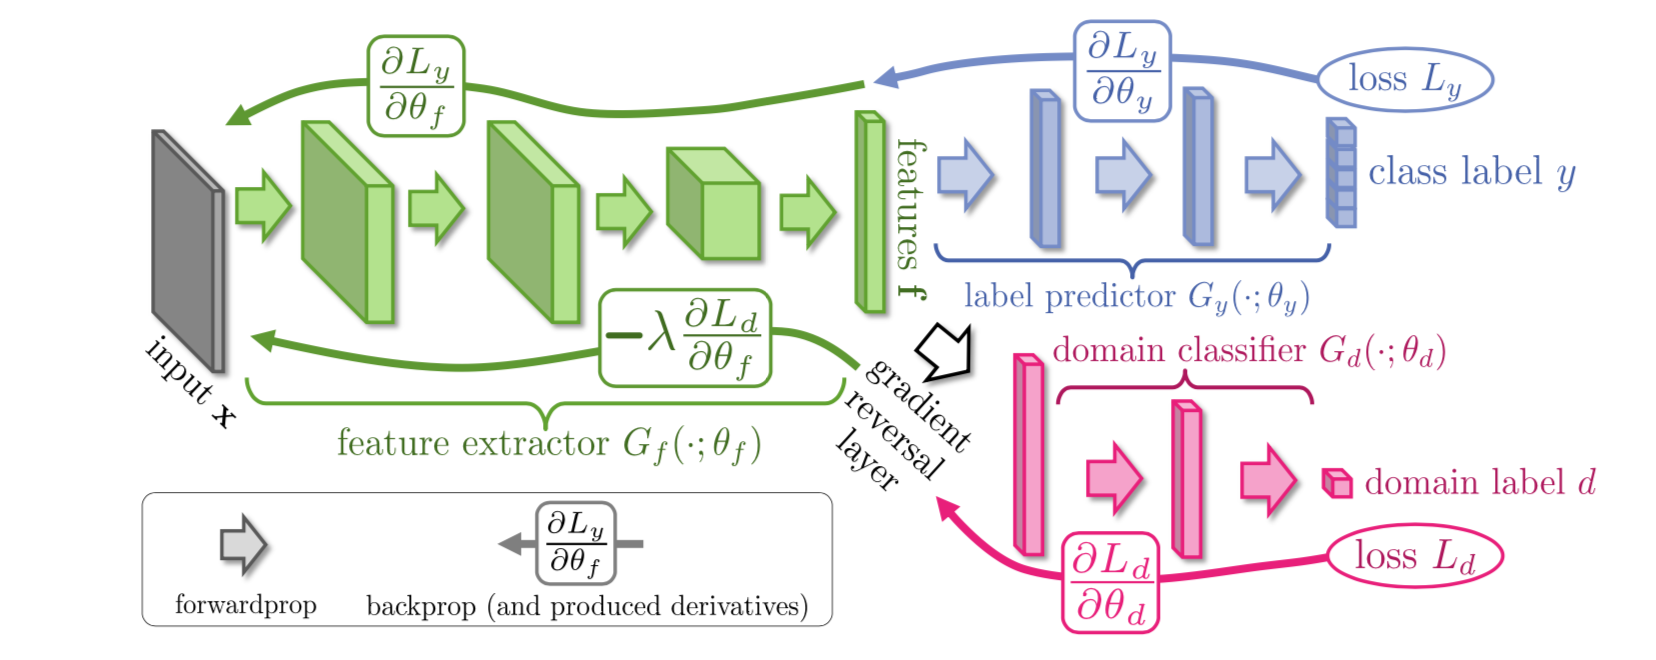
\includegraphics[width=\linewidth]{GRLarch.png}%
    \caption{Architecture with GRL in $G_{d}$ proposed by Ganin and Lempitsky - green part is a \textit{feature extractor} $G_{f}$ that transforms input sample $x$ to feature vector $f$. Afterwards it is classified by \textit{label predictor} $G_{y}$ (blue) and \textit{domain predictor} $G_{d}$ (pink). Picture from author's paper \cite{pmlr-v37-ganin15}.}
    \label{fig:GRLarch}%
\end{figure}

\subsection{Conceptors}
Domain adaptation is a very complex problem, therefore understanding it could be crucial to find some satisfying solutions. As previously mentioned the representation of input sample $x$ after mapping by feature extractor $G_{f}$ is a feature vector $f = G_{f}(x ; \Theta_{f}) \in \mathbb{R}^{D}$. It may be also considered as a point in $\mathbb{R}^{D}$. All the samples from source domain $S$ and target domain $T$ form a point clouds in $\mathbb{R}^{D}$ space that can be denoted as $F_{S}$ and $F_{T}$ respectively:
\begin{align*}
    F_{S} &= \{ G_{f}(x_{s} ; \Theta_{f}) : x_{s} \in S  \} \\
    F_{T} &= \{ G_{f}(x_{t} ; \Theta_{f}) : x_{t} \in T  \}
\end{align*}
\par
If the transformed samples from both domain are considered as points, the feature extractor should find a mapping, that produces as similar point clouds form distributions as possible. Then, the domain classifier could not predict well, if point form $\mathbb{R}^{D}$ with given coordinates belongs to either point cloud $F_{S}$ or $F_{T}$. Obtaining such representation would be a half way to success, as perfect mapping should also place the samples from a single class in the same region for both domains. The label predictor $G_{y}$ would then have to just find a division of the space into the regions for all classes.
\par
It is not a simple task to find a description of points cloud in $\mathbb{R}^{D}$ that would be understandable for a human, if the dimension $D$ is large. Nevertheless, it is possible to approximate these points somehow. One approach is to find an ellipsoid in $\mathbb{R}^{D}$ that captures the majority of the points. This idea was used by Herbert Jaeger to introduce the concpetors \cite{conc}. Such ellipsoid is then used to transform a new point into the cloud of known points. The conceptor is defined as a matrix $C$ that determines an ellipsoid that approximates a given point cloud and is then normalized, so it lies inside the unit sphere. Figure~\ref{fig:conceptor_intro} presents a simple visualization of this idea.
\begin{figure}%
    \centering
    \includegraphics[width=\linewidth]{c_example.png}%
    \caption{Point clouds (black) and conceptors approximating them. Best viewed in color. Picture from "Conceptors: an easy introduction" by Herbert Jaeger \cite{conc_int}. }
    \label{fig:conceptor_intro}%
\end{figure}
Singular vectors of matrix $C$ are the principal axes of the described ellipsoid, while singular values of $C$ are their lengths. They can be easily obtained with SVD method. The conceptor matrix $C$ is obtained with correlation matrix $R = \mathbb{E}_{x}[xx^{T}] \in \mathbb{R}^{N\times N}$ of samples $x \in \mathbb{R}^{N}$ and the aperture parameter $\alpha$, as:
\begin{equation*}
    C = R(R + \alpha^{-2} I)^{-1}
\end{equation*}
\par
The transformation of given point $x$ into the conceptor is made by multiplying it by the matrix $C$. If $x$ lies inside the ellipsoid that is described by the conceptor, the multiplication should act like identity and remain $x$ unchanged. If $x$ is a point from the outside of the ellipsoid then $C$ should move it inside.
\par
As it is possible to represent the high dimensional point cloud with well defined solid shape given by the conceptor, the analysis of $F_{S}$ and $F_{T}$ could be done with operations on these ellipsoids. It may be a good approach to understand the domain adaptation and the influence of GRL.

\section{Research}
\subsection{Paper reproduction}
First stage of all the research made within the thesis was the paper reproduction. All implementations were made with PyTorch \cite{pytorch} - deep learning python framework developed by Facebook. All computations were run on Google Colab \cite{colab} notebook. During most experiments the source domain was MNIST set, while target distribution was MNIST-M. The advanatage of such choice of domains is possibility of quick obtaining a trained model, as architecture needed to classify well MNIST images is not a complex one. Few architectural changes in the network proposed by Ganin and Lempitsky were made, like replacing ReLU activation function with leaky-ReLU \cite{leaky_relu} and using dropout \cite{dropout} during training. The accuracy close to the result from paper (81.49\%) was reached after 30 epochs of training, but already after 10 epochs the 77\% of samples from MNIST-M test set were classified well, while accuracy of domain predictor $G_{d}$ was 68\%. Therefore, a long learning process is not needed to verify if the training may be successful.
\par
The experiments were made when the source and target domains were MNIST and MNIST-M. Very high degree of relatedness between them may  be worrying, therefore the experiment should be verified with some other datasets. One of the others digit image collections is the mentioned previously Street View House Numbers (SVHN) dataset. It was used as source domain, so the label classifier was learned with its samples. MNIST was a target distribution this time.
\par
SVHN is much more complex dataset, with many fuzzy images that presents more than one digit. Therefore obtaining well-performing model requires not only the longer training, but also more advanced architecture. The one used in following experiments had a feature extractor built with 5 convolutional layers, each one using batch normalization \cite{batch_norm} and the leaky-ReLU followed by max pooling and dropout during training process. The class and domian predictors have larger hidden layers than before. This architecture allows us to get reasonable results after about 18 epochs. The model proposed by Ganin and Lempitsky was not that complex, but they trained it for much longer, as for first 150 epochs classification error was high during their research \cite{pmlr-v37-ganin15}.
\par
First training was a basic reproduction of GRL usage. The obtained model classified well 93\% of samples from SVHN test set and 76.5\% images from MNIST test set, slightly higher than best model obtained by the authors (71.07\%). Afterwards, the model built with just a feature extractor and class predictor was learned. The accuracy on SVHN test set was 94\% this time. Despite absence of a domain predictor with GRL, the model managed to recognize well 68\% of MNIST images. Such a well performance on target domain (Ganin and Lempitsky reached 59.19\%) is the result of the complex architecture. Table~\ref{tab:repr_res} shows the composed results of classifying test sets for different domains.
\par
Repeating the experiment with SVHN and MNIST as domains shows, that strong correlation between MNIST and MNIST-M was not the only reason of GRL partial success in domain adaptation. The improvement of the performance beside the model without domain predictor is then really caused by the ability of the network to focus on the semantic of the image - a digit.

\begin{table}
\centering
\begin{tabular}{c|c|c}
\multicolumn{1}{l}{} & \multicolumn{1}{l}{} &  \\
\begin{tabular}[c]{@{}c@{}}Source domain:\\Target domain:\end{tabular}
& \begin{tabular}[c]{@{}c@{}}MNIST\\MNIST-M\end{tabular} & \begin{tabular}[c]{@{}c@{}}SVHN\\MNIST\end{tabular} \\ 
\hline
Accuracy on source domain & 99.12\%~ & 92.42\% \\ 
\hline
\begin{tabular}[c]{@{}c@{}}Accuracy on target domain\\(training without $G_{d}$ with GRL)\end{tabular} & 51.06\% & 68.5\% \\ 
\hline
\begin{tabular}[c]{@{}c@{}}Accuracy on target domain\\(training with $G_{d}$ with GRL)\end{tabular} & 80.57\% & 77.1\%                                              
\end{tabular}
\caption{Classification accuracy for tested domains. Target domain test set was classified with traditional model, as well as with model that uses GRL. The improvement is significant.}
\label{tab:repr_res}
\end{table}

\subsection{Domain information remaining after GRL training}
After reproducing the paper, the next step was to verify if the vector $f=G_{f}(x;\Theta_{f})$ really was domain invariant, as claimed by the authors \cite{pmlr-v37-ganin15}. When model's parameters were tuned a new domain predictor was constructed, this time without the gradient reversal layer. The input for new classifier was a vector $f = G_{f}(x;\Theta_{f})$ for all samples $x$ from both source and target domain, and the goal was to predict which distribution did $x$ come from. So far it was known that $G_{f}$ mapping was incomprehensible for a single domain predictor $G_{d}$ with parameters $\Theta_{d}$, as it's accuracy was just 68\%, while model that returns always 0 (or always 1) would reach 50\%. If the feature extractor mapping really is domain invariant we should not be able to obtain a model with much better performance.
\par
It could have been expected that in fact $G_{f}$ mapping is unclear for just one, used during training, domain predictor. After training the new classifier for just 4 epochs, it managed to predict well the domain of 94\% of examples from MNIST and MNIST-M mapped by $G_{f}$. Also for SVHN and MNIST as distributions, obtaining an almost perfect classifier was a little effort. Therefore we can certainly say, that representation $f$ of input image $x$ still contains a lot of information about the sample's domain, and getting a real domain-shift invariant representation requires much more than just gradient modification during the training. Nevertheless ability to outsmart a single domain predictor significantly improves the model's performance.

\subsection{Adding GRL to well performing domain predictor}
As verified before, feature extractor produces representation that is indistinguishable for a single domain predictor. After the training we can easily obtain a model $G_{d}'$ that successfully predicts the distribution of the sample, if only its architecture does not contain the GRL. It can be checked then, how difficult and effective would be changing the transformation made by $G_{f}$, so it become unclear for the well performing domain predictor $G_{d}'$. The gradient reversal layer is added at the beginning of the classifier's architecture. Then the whole model it trained once again, but now the components are $G_{f}$, $G_{y}$ and $G_{d}'$. 
\par
After just few epochs accuracy of $G_{d}'$ has decreased significantly, as $G_{f}$ mapping adjusted to the new architecture. However, classifying samples from target distribution has not got any better. Also it is not known, how the $G_{d}'$ with GRL differs from $G_{d}$. If in fact both these predictors use highly correlated features to compute their results, then they are almost equal. Moreover, during training the whole model with $G_{d}'$, $G_{d}$ is not used anymore, so we can't say, that $G_{f}$ produces the representation that is unclear for two domain predictors. Maintaining multiple domain classifiers may cause some improvement, however this approach would explain neither how GRL helps in DA task, nor what really is domain adaptation. Therefore it was not implemented.

\subsection{Domain information vanishing}
Absence of domain information in feature vector is highly desirable in domain adaptation problem. Unfortunately GRL does not force such representation, as distribution predictor can be easily obtained - with 16 epochs of training the model achieved 95\% accuracy. Therefore, label classifier prediction is dependent on domain of the input image. Checking how successful can be a domain classifier on class predictor's first layer would show the magnitude of this dependency. 
\par
After 16 epochs of such classifier's training its accuracy in prediction the distribution of the input image was 88\%, then a decay of domain information happened, which improved the performance on target domain. Therefore, the growth of uncertainty of distribution classifier may cause even better results. This leads to the next experiment - "plugging" a domain predictor with GRL to the output of the first layer of class predictor. The weights of feature extractor are frozen now, as we don't want to change its mapping. The task now is to take the transformation, that leaves 88\% of information about the distribution of the input, and try to decrease this result with GRL.
\par
A special architecture of the network was used during thus experiment. Class predictor so far was built with just an input layer and the output layer. This time it was extended with two extra hidden layers. With deeper model we can monitor more precisely the decay of domain information. However, obtaining as high results as the shallow model requires more epochs of training the deeper model. Therefore, the results of consecutive experiments are a bit lower, as the length of the learning process was still short.
\par
When the new domain classifier with GRL was applied to the output of $G_{y}$ first layer, after 16 epochs of training the accuracy on target domain test set slightly increased. To check if the distribution information had vanished even more, the new domain predictor was learned. Its accuracy reached 75\%, therefore applying GRL to the output of the layer had definitely made in more domain invariant. This observation induces to check if the decay of distribution information would advance in deeper layers of the architecture.
\par
After 16 epoch of training the accuracy of the fresh model on the target domain (MINST-M) test set was 78.6\%. Then the feature extractor was frozen and the new distribution classifier (without GRL) was obtained to measure the domain information in $G_{f}$ output. Afterwards the first layer of $G_{y}$ was used just like feature extractor. The new $G_{d}$ with GRL was plugged to its output, therefore, the layer's mapping was used by the rest of class predictor and the domain classifier as well. This should lead to making the layer's output more domain invariant, what was checked with obtaining next distribution predictor. The procedure was then repeated on following layers of $G_{y}$. Table~\ref{tab:domain_vanishing} shows the results of predictors on each stage. Measuring domain information or applying model with GRL on $G_{y}$ output layer would be pointless, as these values are probabilities of each digit. Figure~\ref{fig:domain_v} presents the described learning process.

\begin{table}
\begin{center}
\begin{adjustbox}{width=1.2\textwidth,center=\textwidth}
\begin{tabular}{c|c|c|c|c}
\multicolumn{1}{l}{} & \multicolumn{1}{l}{} & \multicolumn{1}{l}{} & \multicolumn{1}{l}{} & \\
Accuracy of \textbackslash{} model's layer & $G_{f}$ output  & input & ~1st hidden & 2nd hidden \\ 
\hline
Domain classifier on output & 99.99\%~ & 87.86\% & 75.13\% & 69.47\% \\ 
\hline
Domain classifier after adding GRL~ & 95.95\% & 74.75\% & 68.19\% & 68.6\%  \\ 
\hline
\begin{tabular}[c]{@{}c@{}}Target domain test set classification \\(after applying domain predictor with GRL)\end{tabular} & 78.6\% & 78.74\% & 79.06\% & 79.26\%    
\end{tabular}
\end{adjustbox}
\caption{Domain information vanishing research - for output layer of $G_{f}$ and input and both hidden layers of $G_{y}$ firstly the best possible domain predictor is obtained, then the $G_{d}$ with GRL is applied to the layer and accuracy of classifying the target domain test set and sample distribution are measured. While plugging model with GRL to one of the $G_{y}$ layers, the feature extractor and all previous layers of $G_{y}$ are frozen}
\label{tab:domain_vanishing}
\end{center}
\end{table}

\begin{figure}
    \centering
    \vspace*{-3cm}
    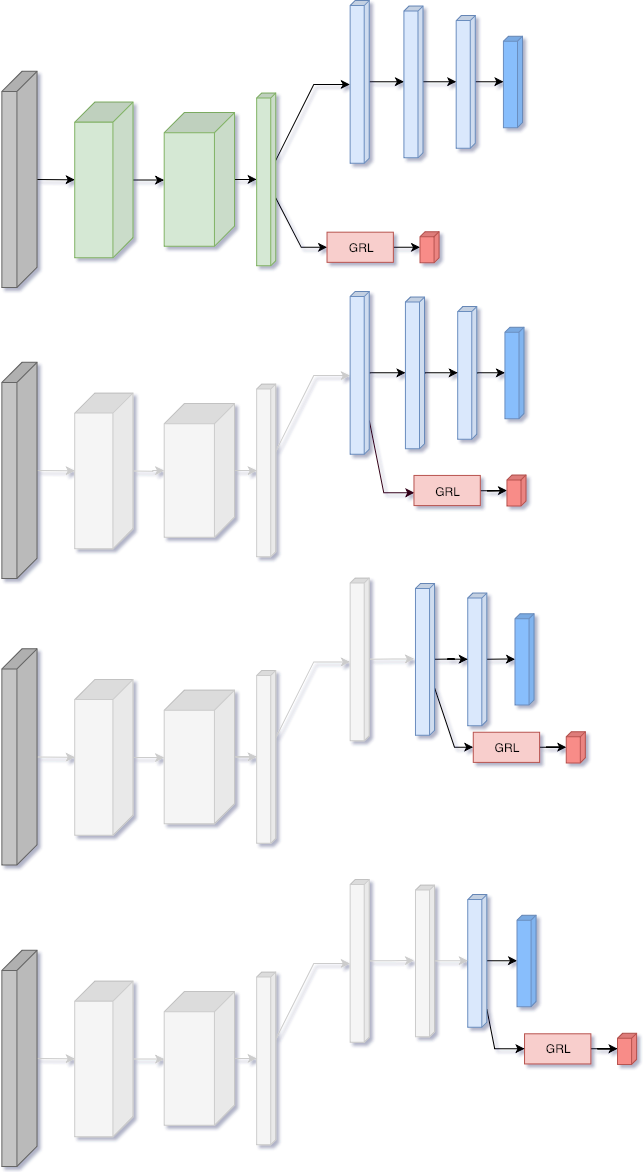
\includegraphics[scale=0.45]{domain_v.png}%
    \caption{Domain information vanishing process. Firstly the domain predictor is plugged to the output of $G_{f}$. Then $G_{f}$ is frozen and model with GRL is applied to the input layer of class predictor. In consecutive stages the layer is frozen, and GRL is plugged to the following one. Green blocks represent $G_{f}$, blue ones $G_{y}$ while pink are domain predictor $G_{d}$. Grey blocks are frozen layers. Best viewed in color.}
    \label{fig:domain_v}%    
\end{figure}

\par
Adding a domain predictor with GRL definitely caused the decay of distribution information, as applying it on $G_{y}$ input layer decreased the accuracy of domain classifier by 15\%. Therefore, the information passed by the first layer of class predictor is not as disturbed by distribution features as before. The experiment shows that applying model with GRL to layers of label classifier makes it more domain invariant. Even though the performance on test set from target distribution did not improve significantly, it seems to be a good practise to apply GRL to more layers.
\par
Vanishing of domain information in deeper layers may be also caused by the complexity of input image transformation on this stage. The small decrease of domain predictor accuracy confirms the small impact of adding model with GRL. It seems like applying an extra domain classifier is more reasonable on early layers of $G_{y}$. It may be helpful observation, if the learning process lasts for a long time. 
\par
The deeper model was not as accurate as the one without any hidden layers in class predictor. Therefore, the experiment was repeated on the smaller model with just a single hidden layer. Each stage of the learning process lasted 16 epochs Plugging the domain classifier to the layer's of this model also caused the decay of distribution information and an improvement on MNIST-M test set. Finally the model reached 80.7\% accuracy on it, while basic model trained for same number of epochs couldn't get higher than 80.57\%. Table~\ref{tab:domain_v_single_hidden} presents detailed results.
\begin{table}
\centering
\begin{tabular}{c|c|c|c}
\multicolumn{1}{l}{} & \multicolumn{1}{l}{} & \multicolumn{1}{l}{} & \\
Accuracy of \textbackslash{} model's layer & $G_{f}$ output & input & ~hidden \\ 
\hline
Domain classifier on output & 99.99\%~ & 89.69\% & 77.43\%  \\ 
\hline
Domain classifier after adding GRL~ & 93.95\% & 78.28\% & 71.83\%  \\ 
\hline
\begin{tabular}[c]{@{}l@{}}Target domain test set classification \\(after applying domain predictor with GRL)\end{tabular} & 76.91\% & 80.6\% & 80.7\%  
\end{tabular}
\caption{Domain vanishing for a model with single hidden layer.}
\label{tab:domain_v_single_hidden}
\end{table}
\par
Applying a new domain predictor with a gradient reversal layer turned out to be a successful modification. Although the improvement of results was small, the inner representations of input data are definitely more domain invariant, therefore it might be crucial in some situations. Also it came out, that if computational cost of applying new classifier to each layer is too high, the best practise is to use it with first layers of the label predictor.

\subsection{Hyperparameters impact}

\subsubsection{Training continuation with increased $\lambda$}
During the training process the $\lambda$ coefficient grows from 0 to 1, as the feature extractor's output should be firstly adjusted to label predictor, and then made more and more domain invariant. When the final model is obtained, parameters $\Theta_{y}$ are well tuned, as accuracy on source domain - MNIST test set is about 99\%. $G_{y}$ is already well trained then, the only limitation is not domain invariant enough transformation made by $G_{f}$. As forcing this invariance is the $G_{d}$ goal, we could try to increase its impact on $G_{f}$ when $G_{y}$ is well trained. Therefore the learning process was repeated with a single modification - $\lambda$ had fixed value, that was greater than 1. In first attempt $\lambda$ was set to 3. After 10 epochs the model had 79.2\% accuracy on MNIST-M test set, for next 10 epochs of training fixed $\lambda$ was used, and the result increased to 80.8\%. If we train a fresh model for 20 epochs with increasing $\lambda$, we would reach comparable accuracy, so we cannot be sure, that the continued training with higher and fixed $\lambda$ will often improve the model's performance. However it seems reasonable to apply this kind of continuation, when larger epochs number does not help.
\par
Setting $\lambda$ parameter to some value grater then 1 is enhancing the impact of domain predictor on feature extractor mapping. However if the coefficient would be too large, it may lead to a decrease of label classifier accuracy. During experiments, when $\lambda = 6$ a pre-trained model gets chaotic, its result fluctuate over the epochs, and does not reach the level from first training. Therefore we should worry about picking the right value for $\lambda$ coefficient during training continuation.

\subsubsection{Tuning model size}
Domain predictor with GRL did not manage to force the network to separate the information about the domain from some digit features. $G_{f}$ mapping satisfies both label and domain predictor, as we can easily obtain a successful domain classifier, so the representation $f=G_{f}(x;\Theta_{f})$ of input sample $x$ is not domain shift invariant. During all previous experiments, feature vector $f$ was 320-dimensional. Maybe the size is so large, that $G_{y}$ uses only its fraction, and the rest of the space is filled with information about the distribution of the input. Therefore a decreasing of $G_{f}$ output size should be considered.
\par
The intuition is that maybe there is an optimal size of feature extractor output. It would be big enough for $G_{y}$ to predict input's label with as high accuracy as with current architecture, but space left unused by class predictor would be too little to be sufficient for any domain predictor. The approach with a domain classifier without GRL should also be tried. If two models would compete for space of feature vector $f$, if it was too small, one of the network would "lose" and had no opportunity to learn.
\par
So far feature extractor was constructed with only convolution layers. During these experiments it was extended by single fully connected layer that was mapping the last convolutional layer's output from $\mathbb{R}^{320}$ to $\mathbb{R}^{D'}$, where $D' = 280, 240, 200, 180, 160, 120$. Then the smaller feature vector was classified by class predictor $G_{y}$ and domain predictor $G_{d}$ containing GRL. 
\par
When feature extractor tries to store all the features in lower dimension, the training process gets noisy. If the number of dimensions $D'$ is too little, value of the loss function may become NaN. It happens if the training lasts for too little epochs, when $\lambda$ gets close to 1 quickly and feature extractor is confused with two different gradients from $G_{y}$ and $G_{d}$. As $G_{f}$ returns just few values, both predictors compete for significant changes in most of them, what lead to the failure of the training. GRL may handicap the learning process then.
\par
After training each architecture the results were not surprising at all. The more complex the model was, the higher accuracy it reached. Moreover, adding fully connected layer caused noticeable fall of performance.  Figure~\ref{fig:size_tune} presents the accuracy of each model. 
\begin{figure}[htb]%
    \centering
    \includegraphics[width=\linewidth]{size_tune.png}%
    \caption{Accuracy of models with different feature extractor output size over the epochs. The \textbf{model 0} is the architecture used during previous experiments, with 320-dimensional $G_{f}$ output. \textbf{model 1 - model 6} are build with feature extractor that is extended with single fully connected layer, which return feature vector in smaller dimension, respectively: 280, 240, 200, 180, 160, 120. Labels present results on MNIST-M test set. We can see, that adding a fully connected layer caused decreasing of model's accuracy. }
    \label{fig:size_tune}%
\end{figure}
\par
When two different models use the feature extractor's output, $G_{f}$ tries to produce the result that would fit for both classifiers. So far GRL was jumbling it with purpose to make $G_{f}$ output clear for label predictor and as impenetrable as possible for domain classifier. If $G_{d}$ doesn't contain a gradient reversal layer, it would act like a regular binary classifier. The feature extractor would then try to return an output that would contain information about both the label of the input, as well as the domain of the sample. Therefore if the $G_{f}$ output would be too small, one of the classifier could receive too little data to learn well. If it would be the domain predictor, then the representation gets more domain invariant.
\par
Once again feature extractor was extended by fully connected layer. This time it maps the feature vector to even 5-dimensional space. The goal was to train $G_{y}$ and $G_{d}$ to reach high accuracy simultaneously. When all the models are learned results are unsatisfactory. In each case both label and domain predictor perform well within their tasks - $G_{y}$ reaches over 98\% accuracy on MNIST test set, even when feature vector $f$ is 5-dimensional. Domain classifier in every architecture is almost always right. However there is an enormous decrease in target domain classifying performance - all the models have accuracy on MNIST-M test set under 20\%, twice less than a simple CNN trained on MNIST.
\par
Such a poor result definitely is a disappointment. Not only all the intuitions were wrong - limiting the output space did not force feature extractor to separate the data, but even model's performance get much worse. It seems that domain predictor's impact on feature extractor is so high, that the $G_{f}$ mapping becomes highly correlated with the distribution of the input, therefore, when we transform sample from target domain its representation is meaningless. Straightforward using of common feature vector mapping for two architectures is not a good idea then.

\subsubsection{Adam Optimizer}
Ganin and Lempitsky used Stochastic gradinet descent (SGD) optimizer during thier research. However, in recent years some fancy optimization methods released and they can boost the training process even more. One of them is Adam Optimizer. It is much more complex than SGD, with individual learning rate for each parameter and usage of more gradient properties. 
\par
To check if Adam may improve our model, the optimizer for each network was changed. After 10 epochs of training accuracy on target domain was slightly higher than before. During a longer training the results obtained by model tuned with Adam were usually higher than when SGD was used. Adam optimizer turned out to be a good choice. Its parameters should be initialized carefully, as during the training the loss may get NaN value much easier. In our particular case, the initial learning rate was reduced from 0.01 for SGD to 0.001 for Adam.

\subsection{Impact of gradient modifications}
Gradient reversal layer is nothing but a simple modification of the gradient. Executed experiments show, that multiplying the gradient by some negative value brings a great improvement in the domain adaptation. The motivation of GRL is producing the domain invariant representation, by following during backpropagation the opposite direction of the domain predictor's gradient. Despite the reality is significantly different, the results are satisfying. Therefore it should be verified, how important for the improvement is transforming the gradient in that particular way, and what is the result of some other modifications.

\subsubsection{Random gradient replacement}
First of tested gradient modifications is replacing the real gradient with some random numbers. Formally, if $Rand()$ is a function returning the random real number from range $(0,1)$, replacing the gradient is:
\begin{equation*}
GradRand_{\alpha}(x, \lambda) = \begin{cases}
x &\text{forward pass}\\
Rand() \cdot \alpha \cdot \lambda &\text{backward pass}
\end{cases}
\end{equation*}
\par
The function is parameterized by $\alpha$ that is scaling the range of random number. Simultaneously multiplying by $\lambda$ is kept, as it is still increasing over the training, to enhance the impact of gradient modification. One could say, that both $\alpha$ and $\lambda$ don't matter as multiplying a random value by some scalar results in a random value, but limiting its range is crucial to avoid training failure.
\par
Used architecture was again built with feature extractor $G_{f}$, label predictor $G_{y}$ and domain classifier $G_{d}$. The only difference is that first layer of $G_{d}$ was a gradient random layer, which was performing $GradRand_{\alpha}$ function. Initially the $\alpha$ was set to 1. After few epochs of training, when $\lambda$ increased above small value, the loss function of the model became NaN. When $\alpha$ was decreased to 0.1 and 0.01, the failure of training repeated. It was needed to use $\alpha = \frac{1}{1000}$ to end up with successful training.
\par
Such a low value of $\alpha$ causes the lack of $G_{d}$ impact on feature extractor. $G_{f}$ was tuning its parameters basing on $G_{y}$ gradient and a little noise from domain predictor, as its gradient was a value from range $(0, \frac{1}{1000})$. Moreover the real gradient of domain classifier is ignored at all, therefore it could not be computed as well. Therefore the results of the model are not surprising - classification of examples from both source domain, which was again MNIST and MNIST-M, was as good as in model without any extra domain predictor. The $G_{d}$ reached very high accuracy in domain predicting, as there was nothing that would disturb it.
\par
Replacing gradient by some random does not seem very effective. Firstly, the random value must be small, otherwise, the training fails. Secondly there was not any improvement of the model. Moreover tuning parameters of $G_{d}$ was an unnecessary computational effort. Nevertheless adding some random values to the real gradient may be considered as an attempt to avoid overfitting, as it may slightly decrease the impact of real data.

\subsubsection{Random gradient multiplying}
Second attempt to modifying the gradient of domain predictor was also based on random values. This time instead of simple replacement, the real gradient was multiplied by some random number. Once again its range was parameterized by $\alpha$ coefficient. The increasing $\lambda$ was also used over training epochs. The modification may be specified as:
\begin{equation*}
GradRandMult_{\alpha}(x, \lambda) = \begin{cases}
x &\text{forward pass}\\
Rand() \cdot \alpha \cdot \lambda \cdot x &\text{backward pass}
\end{cases}
\end{equation*}
\par
The architecture of learned model was changed, so domain predictor was performing $GradRandMult_{\alpha}$ at the beginning. This time using $\alpha = 1$ did not cause the failure of training, but the model's behaviour was simmilar to the situation, when both $G_{y}$ and domain predictor $G_{d}$ without GRL were influencing the feature extractor. Model was effective on source domain test set and managed to predict the distribution of the input, but accuracy on target domain was terrible, just 28\% on the MNIST-M test set. This seems reasonable, as the gradient is now multiplied by some value from range $(0,1)$, while in the case without random number it was always 1. Therefore the bad impact of the domain predictor was slightly lower and the result on target domain is then a bit better, but very unsatisfying.
\par
Afterwards the $\alpha$ was set to 0.1, what considerably improved the previous model. While domain predictor's performance and accuracy on source domain test set kept over 99\%, the result on target distribution increased to 50\%. These results are similar to the score of model without domain classifier. As the impact of $G_{d}$ on feature extractor is rather low, this behaviour could be expected.
\par
Some bigger changes in model's performance could have been noticed if the $\alpha$ parameter was set to a negative value. The model behaved then similarly to the architecture with GRL. If $\alpha = -\frac{1}{10}$ accuracy on MNIST test set kept 99\%, while target domain samples were recognized correctly in 67\%. Moreover the accuracy of $G_{d}$ fell to 81\%. These results shows that the gradient multiplication with such $\alpha$ behaved just like a soft version of GRL.
\par
Afterwards $\alpha$ was set to -1, so the gradient was scaled by negative number from range $(-1, 0)$. As it could have been expected the result was close to the performance of model with GRL - MNIST test set was classified well in 99\%, accuracy on MNIST-M was 76\% and $G_{d}$ result was down to 72\%. The model performed just like it was using GRL, and it seems reasonable.

\subsubsection{Gradient inversion layer}
The reversion of the gradient's direction points at the function maximum. Therefore, the intuition behind GRL is to find such parameters $\Theta_{f}$ of feature extractor, that the domain predictor $G_{d}$ is as incorrect as possible. These parameters can be found if $G_{f}$ tunes them w.r.t. the reversion of $G_{d}$ loss function gradient's direction.
\par
The gradient not only points the direction of function's minimum, but also determines the magnitude of each parameter's impact on final result, as gradient is a multi-variable derivative. Therefore, when the goal is to set such parameters $\Theta_{f}$, that transformation made by $G_{f}$ is absolutely meaningless for domain predictor, reversing the magnitude of gradient's value should be considered. It would cause that crucial changes for $G_{d}$ would be ignored, while parameters that were already well tuned from domain predictor point of view, would be significantly changed. Moreover each value would had its sign changed, so the direction opposite to the one pointing at minimum would be followed. 
\par
Such modification could not only force feature extractor to tune its parameters in a way that loss function of $G_{d}$ gets higher and higher value, but also to disallow the domain predictor from finding any dependencies. If only $G_{d}$ finds pattern in some $G_{f}$ parameters they are changed much more than some irrelevant ones, so no meaningful information about domain would occur in feature extractor mapping. 
\par
The described transformation could be specified as function, which argument is a vector of real values $x = [x_{0}...x_{D-1}]$. Once again during forward pass it remains unchanged, while the modification is made during backpropagation:
\begin{equation*}
GradInverse(x, \lambda) = \begin{cases}
x &\text{forward pass}\\
-\lambda \cdot (\max_{0 \leq i < D} |x_{i}| \dotdiv x) &\text{backward pass}
\end{cases}
\end{equation*}
where $\dotdiv$ is element-wise difference - for each value of the vector $x$ it is subtracted from the largest absolute value from the entire vector.
\par
Such transformation can be inserted at the beginning of the model just like GRL. The computational cost of the training is a bit bigger, as for each input sample the maximum value must be computed. Nevertheless, learning MNIST classification does not take a long time.
\par
Results of the model with domain predictor $G_{d}$ started with $GradInverse$ are promising. 
After just 10 epochs of training the accuracy on MNIST-M test set was 78.87\%. A model with GRL instead of $GradInverse$ managed to get just a bit better result. Moreover, the domain predictor $G_{d}$ classified well only 58\% of all samples, which is much lower than when GRL was used.
\par
Using $GradInverse$ was supposed to decrease the score of the domain classifier by tuning the feature extractor parameters absolutely opposite to its requests. With no doubt model with $GradInverse$ succeed in this task. The accuracy of classifying examples from target domain was a bit lower than with GRL, but inversing the magnitude of the gradient's absolute values definitely is a new option in domain adaptation. The partial success of this approach shows also, that some other gradient modification may cause even better performance than GRL.

\subsection{Other experiments}
\subsubsection{Enforcing Orthogonality}
State of the art domain adaptation approaches reach much higher results than a model with GRL. Therefore looking for some improvement is not groundless. With MNIST as source domain and MNIST-M as target distribution, over 90\% accuracy on MNIST-M test set has been reached \cite{dida}. It should be mentioned that top-performing domain adaptation models apply some data augmentation techniques, which make MNIST more similar to MNIST-M. One of such transformation is adding to the dataset a color-negative version of each sample (white background, black digit) \cite{augm}. During all experiments made within this thesis no augmentation was made.
\par
First attempt was based on some mathematical properties. As feature extractor $G_{f}$ maps input to vector $f \in \mathbb{R}^{D}$ we can treat this vector as a point in D-dimensional space. We want representation $f$ of input image not to depend on its domain, that means, we want get to a situation where domain predictor $G_{d}$ requires some feature dependencies that are omitted by $G_{f}$ mapping, so the only features left are useful for the label predictor. Therefore we want $G_{y}$ and $G_{d}$ to use disjoint sets of data dependencies. Transformation made by each of classifier is in fact matrix multiplication. Predictors contain an input layer, that maps $f \in \mathbb{R}^{D}$ to some $f_{i} \in \mathbb{R}^{I}$. Moreover, multiplying the coordinates of D-dimensional point, represented by $f$, by some matrix is in fact projecting it onto some directions.  As both models take a point from $\mathbb{R}^{D}$ as an input and process it based on some of its coordinates, we can say, that using disjoint dependencies is in fact transforming the input point with some pairwise (between predictors) orthogonal vectors. Then shifting domain means moving the data along directions that are used by domain predictor, which is unnoticeable for class predictor, therefore representation $f$ remains unchanged, as feature extractor ignore dependencies used by $G_{d}$.
\par
The predictor's input layer is a matrix $D \times I$ that determines I directions that matters for the model. We can then verify if predictors use orthogonal set of directions by computing the dot product of both matrices. If it is close to zero, the directions are more independent, so more orthogonal. When we compute the mean of square of dot product values after the model's training, it turns out to be a very small number. Therefore directions of $G_{y}$ and $G_{d}$ are almost orthogonal. It may be a good idea to use this learned model and train it again, with modified loss function, that would force $G_{y}$ and $G_{d}$ to minimize that dot product even more. We can add to the objective the mean of square of predictors matrices dot product, i.e. if we denote loss function as $E(\Theta_{f}, \Theta_{y}, \Theta_{d})$ and input layer matrices of classifiers as $W_{I_{y}}$ and $W_{I_{d}}$, then new loss function is:
\begin{equation*}
E'(\Theta_{f}, \Theta_{y}, \Theta_{d}) = E(\Theta_{f}, \Theta_{y}, \Theta_{d}) + \overline{(W_{I_{y}} \cdot W_{I_{d}}^{T})^{2}}
\end{equation*}
\par
The new loss function caused reducing of the dot product indeed, but it had no impact on model's performance. As new loss is punishing for product of model's weights the optimizer may force them to decay - lower values implies lower product. This would be undesirable, we want the dot product to reduce not because of shorter vectors, but because of their orthogonality. However monitoring the average length of these vectors shows that they are not shrinking. 
\subsubsection{Weight decay}
It is not sure, how important preventing the decay of the predictors' matrices weights is necessary, so the model was forced to test it by minimizing the lengths of vectors composed in $W_{i_{y}}$ and $W_{i_{d}}$ as much as possible. When only the new loss with weight regularization was applied, these values quickly got close to zero. However it did not make the model performance worse, the accuracy over the epochs get even more stable.
\par
Extending the loss function in order to increase orthogonality of directions used by label and domain classifiers did not improve the model's performance. We could notice that before adding new components to loss function, these directions already were almost orthogonal, as GRL's task is to force the predictors to use disjoint features of their common input. The experiment shows that inverting the sign of gradient is the only modification that improves the performance of model with gradient modification. Also applying the weight decay turned out to be a good optimization practice, as it helps to avoid overfitting of the model.

\subsection{Cloud point shape analysis and visualizations}
\subsubsection{Conceptors}
As previously mentioned, feature vectors for all the samples from both domain can be considered as two point clouds $F_{S}$ and $F_{T}$, that can be approximated with ellipsoids afterwards. These ellipsoids are described by the conceptors matrices $C_{S}$ and $C_{T}$. The quality of the feature extractor $G_{f}$ mapping may be measured as the similarity of ellipsoids approximating $F_{S}$ and $F_{T}$, as a domain invariant transformation produces the same point cloud for both distributions. Measuring the similarity of $F_{S}$ and $F_{T}$ can be done by conceptors comparison. 
\par
As conceptor always lies inside an unit sphere, it can be measured, how much of space does it occupies. If the point cloud is scattered over the whole space then it would not be possible to approximate it with nothing but a sphere. However, if points are located in an organized cluster, they can be captured with much more limited ellipsoid. Therefore, the \textit{quota} value measures the fraction of the space that is taken by a conceptor. It can be computed as:
\begin{equation*}
    Q(C) = \frac{1}{N} \sum_{i=1}^{N}{s_{i}}
\end{equation*}
where $s_{i}$ are singular values of conceptor matrix $C$. Moreover, logic operations  can be applied to the conceptors, such as $\neg, \vee, \wedge$. The negation of conceptor is the space orthogonal to the ellipsoid, the disjunction is a conceptor that is obtained with sum of samples sets, while the conjunction is the conceptor that approximates the intersection of these sets. Figure~\ref{fig:conceptor_logic} charts these operations.
\begin{figure}%
    \centering
    \includegraphics[width=\linewidth]{c_logic.png}%
    \caption{Logic operations on 2-dimensional conceptors. Picture from \cite{overc}.}
    \label{fig:conceptor_logic}%
\end{figure}
\par
To assess the similarity of two point clouds corresponding conceptors $C_{S}$ and $C_{T}$ should be computed firstly. Then $C_{S} \vee C_{T}$ is their intersection. The value $Q(C_{S} \vee C_{T})$ determines its magnitude. If it is close to both $Q(C_{S})$ and $Q(C_{T})$ then ellipsoids that approximate both point clouds are similar. The quota of conjunction $Q(C_{S} \wedge C_{T})$ should also be close to the $Q(C_{S} \vee C_{T})$, as intersection of these point clouds should include most of them.
\par
Reliable result demands well computed conceptors. The final values of matrix $C$ depend on the magnitude of the scaling parameter $\alpha$, called the aperture. If it is too low, the conceptor acts as zero mapping, while when the aperture is getting larger, the conceptor matrix becomes an identity matrix, therefore, finding the right aperture is crucial. Jaeger propose some methods for analytical finding the right value of $\alpha$ \cite{conc} for an echo-state network, which can be used if needed.
\par
Described approach was used to measure the similarity of $F_{S}$ and $F_{T}$ point clouds. The domains were MNIST and MNIST-M, and feature extractor $G_{f}$ was mapping an input image to 320-dimensional feature vector $f$, so the conceptor matrices were $C_{MNIST} \in \mathbb{R}^{320\times N}$ and $C_{MNIST-M} \in \mathbb{R}^{320\times N}$, where $N$ was the dataset size. Computational cost of obtaining these matrices is low, even for $N=60000$ samples from dataset, therefore many different setups may be tested.
\par
Xu He and Herbert Jaeger published the paper "Overcoming Catastrophic Interference using Conceptor-Aided Backpropagation" \cite{overc}, where conceptors are used to enable a neural network to learn MNIST and its permutations. Their goal is to obtain a model, that is already trained for some tasks and make it perform well on another one, without an accuracy deacrease for previously learned problems. During the training process the conceptor $A$ describes the space taken by learned tasks. The $Q(A)$ value is monitored during the training, as it determines the ability to learn a new task by the model. When $Q(A)$ gets 1 there is no spare space, and trying to fit any other dataset fails. 
\par
As Xu He and Jaeger use MNIST as their main dataset and receive some satisfying results it seems reasonable to use the same aperture $\alpha$ as the authors. For most of experiments in their paper, the $\alpha$ was set to 4. When such value was used to compute the $C_{MNIST}$ and $C_{MNIST-M}$ conceptors, their quota values were both over $0.99$. This was highly undesirable, as it implied that the points form both point clouds were scattered over the space, therefore the ellipsoids approximating them were not a good depiction. Even the value $Q(C_{MNIST} \vee C_{MNIST-M} )$ and $Q(C_{MNIST} \wedge C_{MNIST-M} )$ were close to each other and to quotas of each conceptors, it did not mean the $F_{MNIST}$ and $F_{MNIST_M}$ were similar. We could only conclude that points from these cloud lied in many regions of the space. 
\par
The lower value of $\alpha$ was used, but for any $\alpha > 1$ the quota of conceptor was over $0.99$, to obtain $Q(C_{MNIST}) < 0.9$ it was needed to set $\alpha = 0.4$. With such low aperture it is hard to say if the results are reliable, as in all experiments made by Xu He and Jaeger, the $\alpha$ was much larger. However, for all tested values, the $Q(C_{MNIST})$ and $Q(C_{MNIST-M})$ were close.
\par
The only interesting result was obtained when the model was trained without the domain predictor $G_{d}$. When the parameters of the model depended only on MNIST samples, the $Q(C_{MNIST})$ was as high as in previously described case, for any $\alpha > 1$ it was over $0.99$. However when $C_{MNIST_M}$ was computed, the quota of the conceptor was clearly lower. As $F_{MNIST-M}$ may be captured with a smaller ellipsoid, then it must be different from $F_{MNIST}$, so classification the MNIST-M samples is much less accurate. Figure~\ref{fig:Q(C)} presents the quota values of $C_{MNIST}$ and $C_{MNIST_M}$ when aperture was in range $[0.1, 1]$.

\begin{figure}
    \centering
    \begin{subfigure}[b]{0.48\textwidth}
        \includegraphics[width =\textwidth]{Q(C).png}
        \caption{Model trained with GRL}
    \end{subfigure}%
    \begin{subfigure}[b]{0.48\textwidth}
        \includegraphics[width =\textwidth]{Q(C_nogrl).png}
        \caption{Model trained without GRL}
    \end{subfigure}%        
    \caption{Quota of concpetors $C_{MNIST}$ (blue) and $C_{MNIST_M}$ (green) for training with or without domain predictor with GRL.}%
    \label{fig:Q(C)}%
\end{figure}
\par
Jaeger proposes conceptors as a way to transform a given point into the well trained by the model point cloud \cite{conc}. This idea sounds attractive for domain adaptation. After computing the conceptor $C_{S}$ for data cloud $F_{S}$, while input sample $x$ would be classified, its feature vector $f = G_{f}(x ; \Theta_{f})$ could be multiplied by $C_{S}$ before processing by $G_{y}$. This would transform it into data cloud that is already well known for the label predictor. Therefore the probabilities for each class would be computed as:
\begin{equation*}
  P(x) =  G_{y}( G_{f}( x ; \Theta_{f} ) \cdot C_{S} ; \Theta_{y} )    
\end{equation*}
Even though this approach was successful with echo-state network, it did not improve the pre-trained model's performance. The $F_{S}$ and $F_{T}$ point clouds were probably similar enough to had almost equal conceptor matrices, therefore multiplying a point form $F_{T}$ by $C_{S}$ was close to identical mapping. Therefore, using conceptors for model's improvement was ineffectual.

\subsubsection{Visualization}
Comparing the $F_{S}$ and $F_{T}$ did not succeed with the conceptors. The knowledge about these point clouds could be helpful in understading the problem of domain adaptation as well as the gradient reversal layer. Therefore we could try to visualize them by setting the size of feature extractor to 3. The $G_{f}$ mapping would be then a function $\mathbb{R}^{M} \rightarrow \mathbb{R}^{3}$, where M is the dimensionality of input sample $x$. Such mapping can be obtained by extending the original feature vector by a single fully connected layer that transforms the feature vector $f \in \mathbb{R}^{D}$ to $\mathbb{R}^{3}$. This kind of feature extractor may be denoted as $G_{3}$ with parameters $\Theta_{3}$. When each point in $F_{S}$ and $F_{T}$ is a 3-dimensional feature vector, its values may be treated as the coordinates, so the point cloud can be easily drawn.
\subsubsection{MNIST and MNIST-M visualizations}
Training model with such a small layer inside is much more difficult task, as many information may be lost during mapping do $\mathbb{R}^{3}$. Therefore, at the beginning the domain classifier $G_{d}$ with GRL was not used. The source domain was MNIST and the target distribution MNIST-M, so the corresponding point clouds might be denoted as $F_{MNIST}$ and $F_{MNIST-M}$. The model achieved 98\% accuracy on the MNSIT test set, but it performed poorly on MNIST-M, just 31\% of digits, were classified well. As parameters of $G_{3}$ were tuned, the point clouds could be visualized. Figure~\ref{fig:MNIST_3D}(a) shows the result of mapping by $G_{3}$ all samples from MNIST test set (blue) and MNIST-M test set (gray). The shape of both point clouds resemble a multi-armed star. Moreover it seems like $F_{MNIST}$ is just a stretched version of $F_{MNIST-M}$. We can expect that each arm contains mapped pictures of same digit. Figure~\ref{fig:MNIST_3D}(b) presents distribution of the images of zero digit from both domains. In both cases the pictures transformations form corresponding arm of the star.
\par
\begin{figure}[htb]%
    \centering
    \begin{subfigure}[b]{0.48\textwidth}
        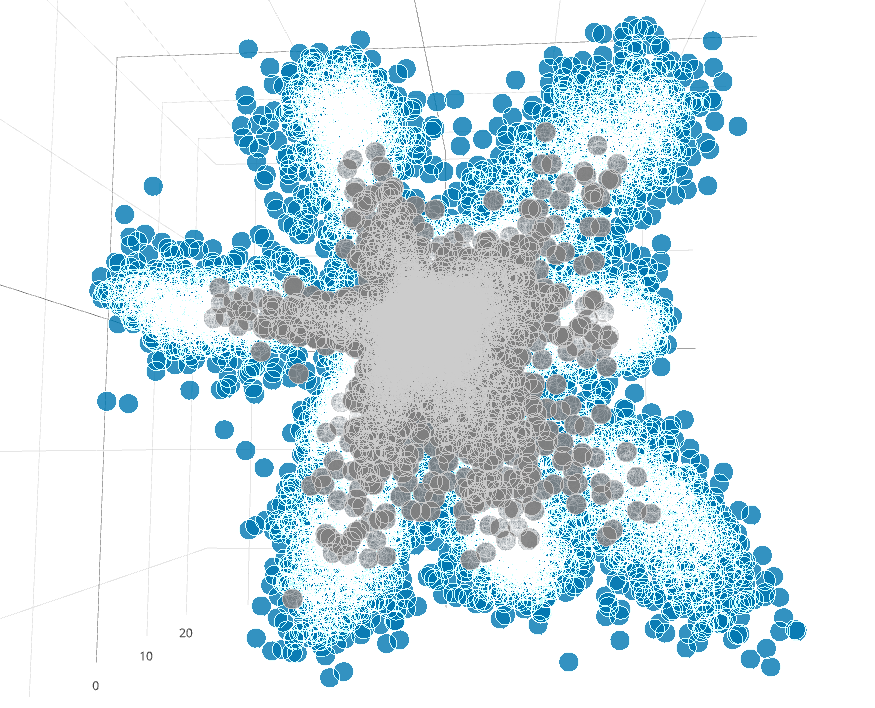
\includegraphics[width =\textwidth]{MNIST_MNISTM.png}
        \caption{MNIST and MNIST-M}
    \end{subfigure}%
    \begin{subfigure}[b]{0.48\textwidth}
        \includegraphics[width =\textwidth]{Zeros_MNIST_MNISTM.png}
        \caption{Zero digit samples}
    \end{subfigure}%    
    \caption{The visualization of samples transformed by feature extractor $G_{3}$. (a) presents two stars formed by samples from source domain (MNIST/blue) and a target domain (MNIST-M/gray) (b) shows how pictures of zero digit are mapped - yellow points are zeros from MNIST and green ones from MNIST-M}%
    \label{fig:MNIST_3D}%
\end{figure}

\subsubsection{GRL visualizations}
As the previous visualization shown, $F_{S}$ and $F_{T}$ are quite similar. It could be expected, that learning the model with GRL should make these point clouds even closer. The model was composed with feature extractor $G_{3}$, label predictor $G_{y}$, and domain classifier $G_{d}$ with GRL. After the training the model got 96\% accuracy on source domain test set and 40\% accuracy on target domain test set. The improvement was almost 30\% in relation to the model without GRL.
\par
The visualization of both point clouds mapped by $G_{3}$ is really surprising.  Figure~\ref{fig:GRL3D} shows how samples from source and target domain were transformed. The second picture presents samples from both distributions. The target domain point cloud $F_{MNIST-M}$ formed a blob that is not similar to the source domain distribution $F_{MNIST}$ at all. The last picture shows the location of zero digit images.

\begin{figure}[htb]%
    \centering
    \begin{subfigure}[b]{0.33\textwidth}
        \includegraphics[width =\textwidth]{GRL_3D1.png}
    \end{subfigure}%
    \begin{subfigure}[b]{0.33\textwidth}
        \includegraphics[width =\textwidth]{GRL_3D2.png}
    \end{subfigure}%
    \begin{subfigure}[b]{0.33\textwidth}
        \includegraphics[width =\textwidth]{GRL_3D3.png}
    \end{subfigure}%   
    
    \caption{Output of $G_{3}$ mapping when GRL was used during training. First picture presents how source domain samples are transformed, second one shows the point clouds for both source (blue) and target (gray) domain. Last picture shows how points with 0 label are distributed.}%
    \label{fig:GRL3D}%
\end{figure}
\par
Training process is very noisy, when feature extractor output is so small. The results after different runs were very diverse. The training often failed when the loss became NaN, the variance of model's accuracy over many training was high. Mapping the feature vector to just 3 numbers caused the loss of many information. Every single training reached its best accuracy after one of the firsts epochs, that are characterized with lower $\lambda$ coefficient. Therefore, to avoid the failure of training process, the $\lambda$ was set to fixed value $\lambda = 0.3$. This allowed the model to perform well, the accuracy on target domain test set was over 50\%.  Figure~\ref{fig:GRL_digits} shows how the input images of particular digits were mapped by feature extractor $G_{3}$. Each arm of star formed by $F_{MNIST}$ corresponds to individual digit. In blob formed by $F_{MNIST-M}$ we can see a cluster for each digit, but it still looks like shuffled. Last picture presents the distribution of both point clouds.

\begin{figure}%
    \centering
    
    \begin{subfigure}[b]{0.33\textwidth}
        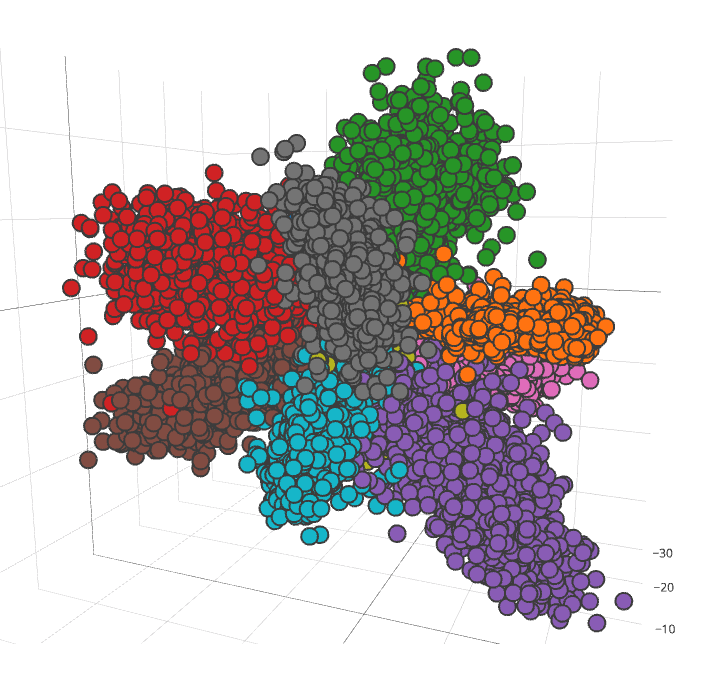
\includegraphics[width =\textwidth]{GRL_digits1.png}
        \caption{$F_{MNIST}$}
    \end{subfigure}%
    \begin{subfigure}[b]{0.33\textwidth}
        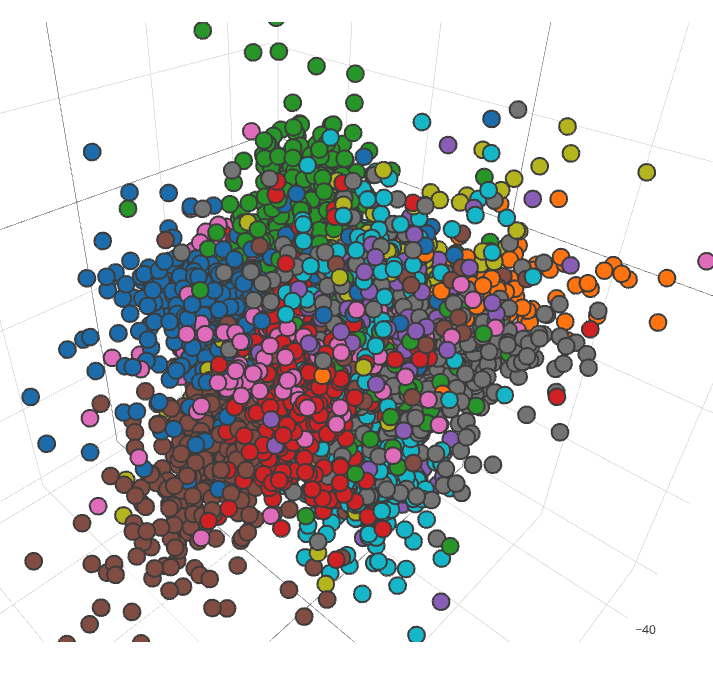
\includegraphics[width =\textwidth]{GRL_digits2.png}
        \caption{$F_{MNIST-M}$}
    \end{subfigure}%
    \begin{subfigure}[b]{0.33\textwidth}
        \includegraphics[width =\textwidth]{GRL_digits3.png}
        \caption{Both point clouds}
    \end{subfigure}%

    \caption{Mapping of the input images of particular digits. The model was learned with GRL and fixed value $\lambda = 0.3$}%
    \label{fig:GRL_digits}%
\end{figure}

\par
To make the plots even more understandable, the feature vector may returns a 2-dimensional feature vector $f \in \mathbb{R}^{2}$. Firstly the model was learned without applying GRL. Although finding the right parameters got even more difficult, after few epochs of training the accuracy on MNIST test set was 95\% and 31\% on the samples from MNIST-M test set. Figure~\ref{fig:2D} presents the $F_{MNIST}$ and $F_{MNIST-M}$ mapped to $\mathbb{R}^{2}$. The point clouds formed multi-armed star again. Each star has less arms than number of classes in the dataset, therefore few of them are stacked in the middle. Classifying of these samples is likely much less accurate. Moreover, majority of points from $F_{MNIST-M}$ lies close to the middle of the coordinate system. As input images of different digits are represented by similar numbers, the classifier cannot be sure while predicting their label.
\par
When GRL was applied during the training, the accuracy on the MNIST-M was much higher, 42\% of sample from target domain were classified well. The last picture of figure~\ref{fig:2D} presents the distribution of $F_{MNIST-M}$ after such training. The samples formed a blob, therefore the better performance is incomprehensible. 

\begin{figure}[htb]%
    \centering
    
    \begin{subfigure}[b]{0.33\textwidth}
        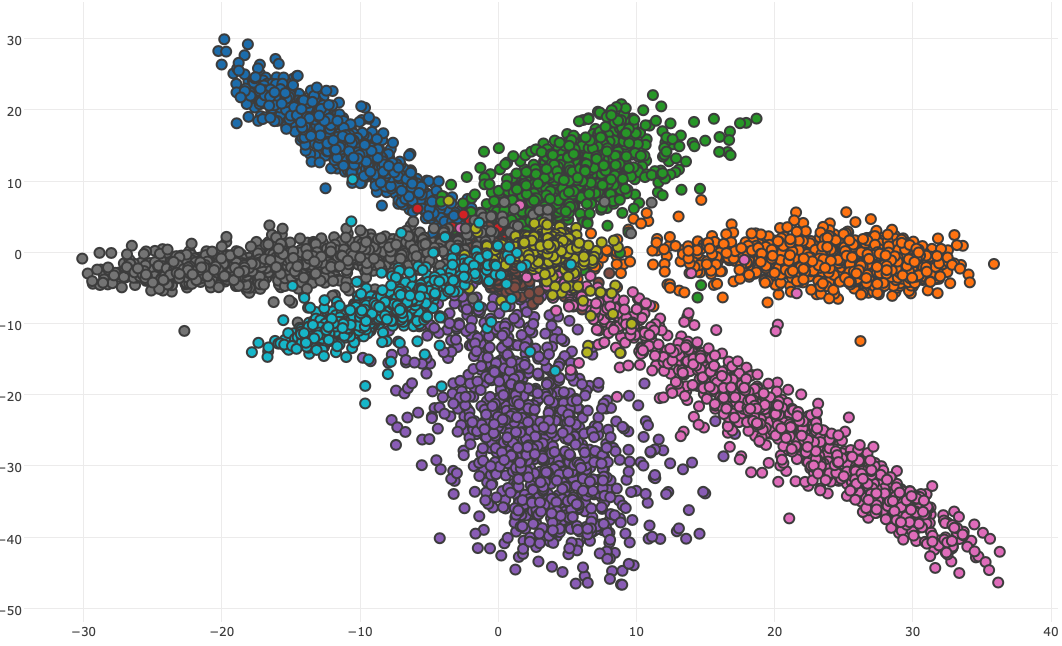
\includegraphics[width =\textwidth]{MNIST_2D.png}
    \end{subfigure}%
    \begin{subfigure}[b]{0.33\textwidth}
        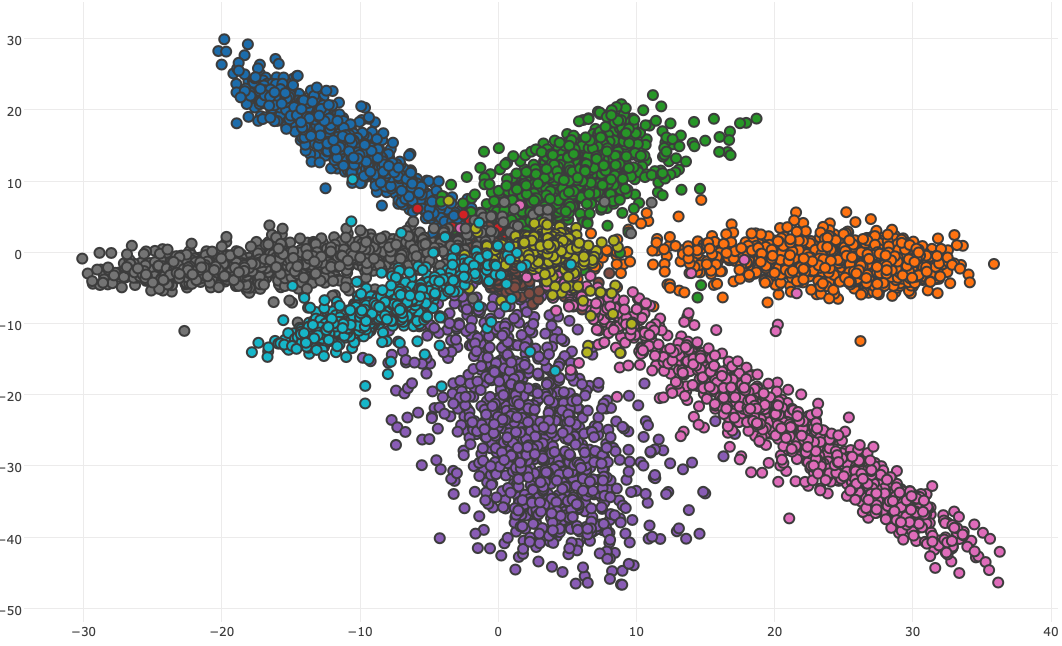
\includegraphics[width =\textwidth]{MNIST_2D.png}
    \end{subfigure}%
    \begin{subfigure}[b]{0.33\textwidth}
        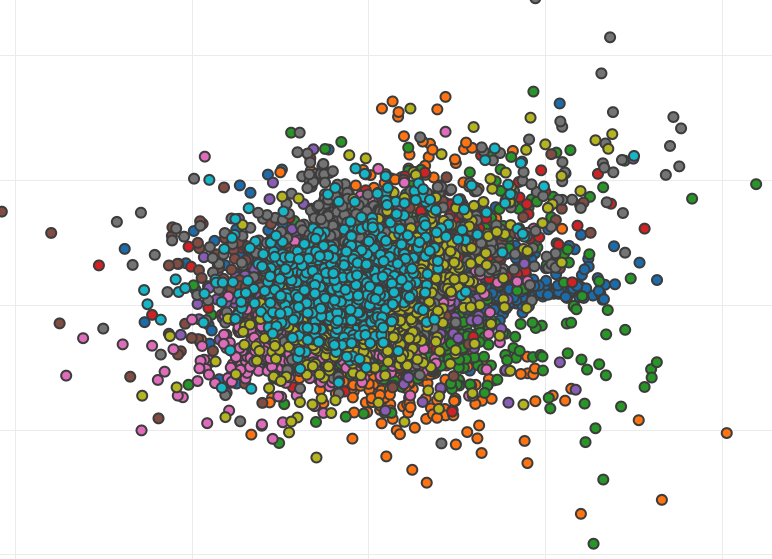
\includegraphics[width =\textwidth]{MNIST_M_2D_GRL.png}
    \end{subfigure}%   
    
    \caption{2-dimensional feature vector mapping. First picture shows the distribution of samples from source domain, second one presents the $F_{MNIST-M}$ without applying GRL during training, while the last image shows $F_{MNIST-M}$ when GRL was used.}%
    \label{fig:2D}%
\end{figure}

\subsubsection{SVHN visualizations}
\par
Visualizing the point cloud $F_{SVHN}$ formed by samples from SVHN dataset mapped by feature vector $G_{3}$ is much more challenging. SVHN images are more complex than MNIST pictures, so compressing the information required to a good classification into just 3 values is a tough mssion. Even without applying GRL during the training, it seems unlikely to obtain a well tuned feature extractor $G_{3}$. Fortunately, a model with a complex $G_{3}$ architecure reached 92\% accuracy on source domain (SVHN) test set classification and 65\% on target domain (MNIST) samples. The performance on MNIST test set is satisfying, the majority of the information was not lost during mapping to $\mathbb{R}^{3}$. Figure~\ref{fig:SVHN_3D} presents the visualization of $F_{SVHN}$ and $F_{MNIST}$ after mapping by $G_{3}$.

\begin{figure}[htb]%
    \centering
    
    \begin{subfigure}[b]{0.33\textwidth}
        \includegraphics[width =\textwidth]{SVHN.png}
        \caption{$F_{SVHN}$}
    \end{subfigure}%
    \begin{subfigure}[b]{0.33\textwidth}
        \includegraphics[width =\textwidth]{SVHN_and_MNIST.png}
        \caption{$F_{MNIST}$}
    \end{subfigure}%
    \begin{subfigure}[b]{0.33\textwidth}
        \includegraphics[width =\textwidth]{Zeros_SVHN_MNIST.png}
        \caption{Zero digit samples}
    \end{subfigure}%

    \caption{The visualization of samples transformed by $G_{3}$. (a) presents the mapping of source domain $F_{SVHN}$, (b) shows also how data from target domain (gray) is mapped into $F_{MNIST}$ and (c) how images of zero digit from source (red) and target (green) domains are distributed.}%
    \label{fig:SVHN_3D}%
\end{figure}
\par
The point cloud $F_{SVHN}$ obtained by $G_{3}$ mapping also formes a shape that resebles multi-armed star. It also looks much sharper than the shapes from previous section. The second picture of figure~\ref{fig:SVHN_3D} presents the distribution of both $F_{SVHN}$ and $F_{MNIST}$. The point clouds are much more similar this time, what is related to the better performance of the model on target domain. The last picture of the figure shows the distribution of zero digit images from both domains. Samples from source domain (red) forms an indvidual arm of the star, while input images from target domain (green) are scattered over two different arms, as well as many of them lie in the middle of the obtained star. It causes the imprecission of classifying the target domain test set, as samples with different labels have very similar feature vectors.
\par
Figure~\ref{fig:SVHN_Digits} shows the distribution of each digit samples after mapping by $G_{3}$. Images of every digit from SVHN formed a sharp, individual arm, while pictures from target domain are a bit mixed, with many of the samples close to the middle of the coordinate system. Therefore classifying a sample by its location in the star formed by the point cloud may be unsuccessful.

\begin{figure}[htb]%
    \centering
    \begin{subfigure}[b]{0.48\textwidth}
        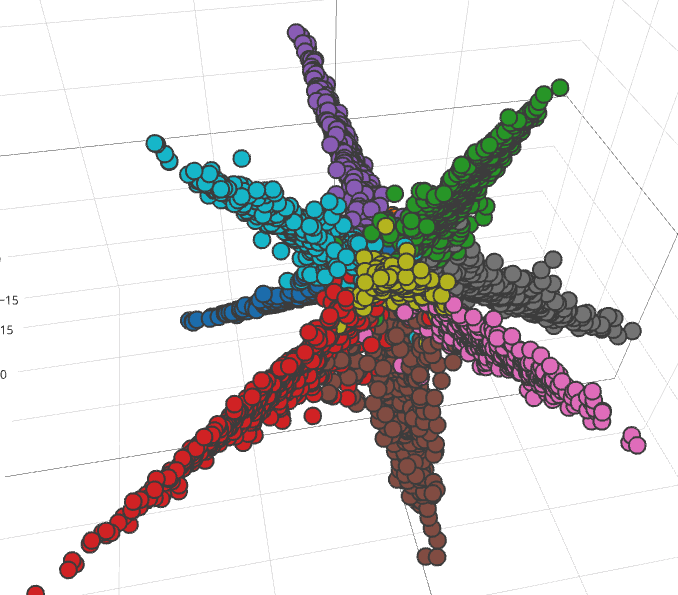
\includegraphics[width =\textwidth]{SVHN_digits1.png}
        \caption{$F_{SVHN}$}
    \end{subfigure}%
    \begin{subfigure}[b]{0.48\textwidth}
        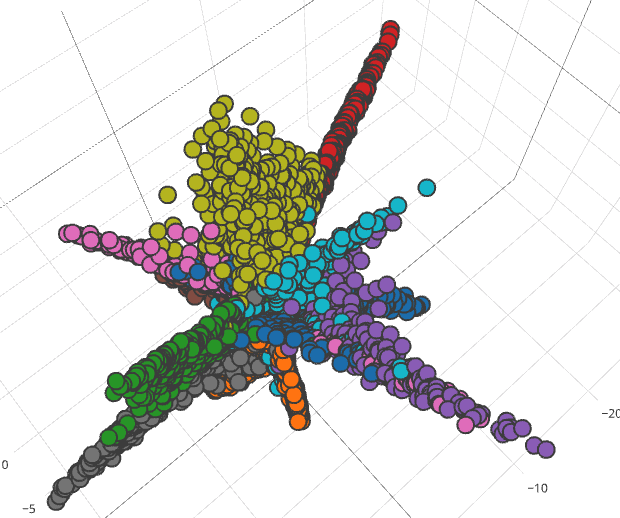
\includegraphics[width =\textwidth]{SVHN_digits2.png}
        \caption{$F_{MNIST}$}
    \end{subfigure}%        
    \caption{Distribution of particular digit images after $G_{3}$ mapping.}%
    \label{fig:SVHN_Digits}%
\end{figure}
\par
Training with GRL applied was very unstable with previous domains. Therefore, it was not surprising that with SVHN as source domain, applying GRL during training a fresh model caused the failure of the learning process. Even if $\lambda$ was set to a fixed small value, the loss function became NaN, it was not possible to get a new model with GRL applied. Nonetheless, the already trained model could be extended with a domain predictor $G_{d}$ with GRL plugged to the output of the feature extractor. After just few epochs of the training, accuracy on target domain test set was 73\%, therefore applying GRL increased the model's performance by 12\%. Unfortunately, the loss function became NaN at a later stage of the learning process. Once again $\lambda$ parameter had to be fixed and small to avoid the training failure. With $\lambda = 0.2$ the model managed to tune its parameters well. Figure~\ref{fig:SVHN_GRL} presents the distribution of both point clouds mapped by $G_{3}$ after the posterior training with GRL applied. This time the target domain samples did not formed a blob, however, the GRL impact on the entire model was much lower in this case. The multi-armed star formed by $F_{SVHN}$ is not as sharp as previously. Also samples from the $F_{MNIST}$ are less mixed, and the point cloud itself is more similar to the $F_{SVHN}$.

\begin{figure}[htb]%
    \centering
    \begin{subfigure}[b]{0.48\textwidth}
        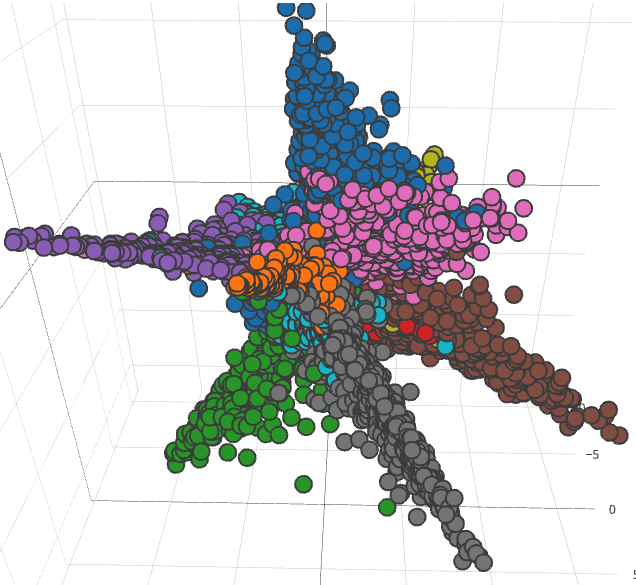
\includegraphics[width =\textwidth]{SVHN_GRL.png}
        \caption{$F_{SVHN}$}
    \end{subfigure}%
    \begin{subfigure}[b]{0.48\textwidth}
        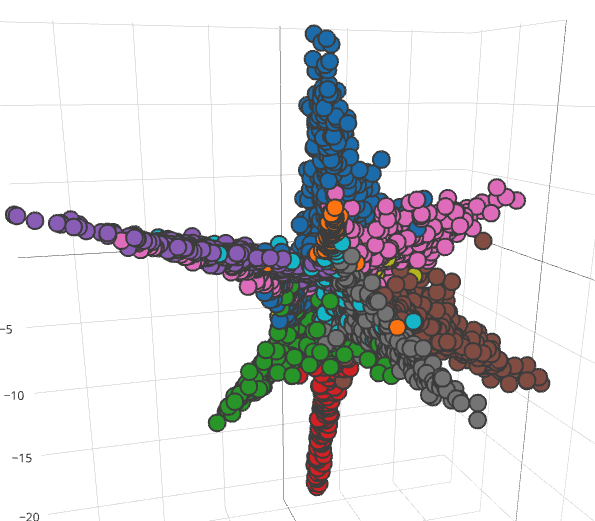
\includegraphics[width =\textwidth]{SVHN_GRL2.png}
        \caption{$F_{MNIST}$}
    \end{subfigure}%        
    \caption{Distribution of particular digit images after $G_{3}$ mapping, when GRL was used during the training.}%
    \label{fig:SVHN_GRL}%
\end{figure}

\subsubsection{3-dimensional layer in class predictor}
Such a restrictive limitation of the feature vector $f$ dimensionality caused a serious decline of model's performance. Also using GRL during training was unsettled, as the learning process often failed. Therefore the layer with the ouput size 3 could be placed in the class predictor, rather than as the last layer of the feature extractor. This approach favours also the training with GRL, as the gradients from both predictors influence a D-dimensional feature vector. The new architecture is then build with feature extractor $G_{f}$ that produces the feature vector $f \in \mathbb{R}^{D}$, domain predictor $G_{d}$ with GRL and the class predictor $G_{y}^{3}$ with a single hidden layer of size 3. 
\par
This architectural change cuased a significant improvement of model's performance. After just 10 epochs of training, the accuracy on target domain, which was MNIST-M, reached 69.08\%, what was much closer to the results obtained by the model with no architectural limitations. To visualize the input sample $x$, it is firstly transformed by $G_{f}$ to feature vector $f \in \mathbb{R}^{D}$ and then mapped by the first layer of class predictor $G_{y}^{3}$ to a 3-dimensional vector $f_{3} \in \mathbb{R}^{3}$. Therefore, the point clouds $F_{MNIST} \in \mathbb{R}^{D}$ and $F_{MNIST-M} \in \mathbb{R}^{D}$ need to be mapped by the first layer of label classifier to be visualized. Figure~\ref{fig:vis_class_pred} presents the result of such mapping. Both point clouds again formed multi-armed stars, but they are much more similar in this case. Also applying GRL did not resulted in transformation of the target domain point cloud to a blob. Using $G_{y}^{3}$ instead of $G_{3}$ is definitely a better approach to visualize the data.
\begin{figure}[htb]%
    \centering
    \begin{subfigure}[b]{0.48\textwidth}
        \includegraphics[width =\textwidth]{bv1.png}
        \caption{Point clouds mapped to $\mathbb{R}^{3}$}
    \end{subfigure}%
    \begin{subfigure}[b]{0.48\textwidth}
        \includegraphics[width =\textwidth]{bv2.png}
        \caption{Digits from MNIST mapped to $\mathbb{R}^{3}$}
    \end{subfigure}%        
    \caption{Mapping of $F_{MNIST}$ and $F_{MNIST-M}$ to $\mathbb{R}^{3}$ by class predictor's first layer. First picture presents both point clouds - blue is the mapping of $F_{MNIST}$, gray is $F_{MNIST-M}$. The second image shows the distribution of each digit from MNIST. Once again the mapped sampled formed a multi-armed star.}%
    \label{fig:vis_class_pred}%
\end{figure}
\par
As visualizations with $G_{y}^{3}$ seem more reliable it can be used to some other analysis. Some of the input images are mapped close to the middle of the coordinate system. As samples from different classes are mixed there, they are likely wrongly classified. Therefore, the distribution of samples with worst and best prediction could be checked. Figure~\ref{fig:best_pred} presents the location of samples that are classified well, and the model is mostly certain to their label. All of these points lie in the peaks of the arms corresponding to their digit. The second picture shows the distribution of these samples as also the misclassified ones. It confirms than mapping the input into the middle area may cause the mistake during classification.
\begin{figure}[htb]%
    \centering
    \begin{subfigure}[b]{0.48\textwidth}
        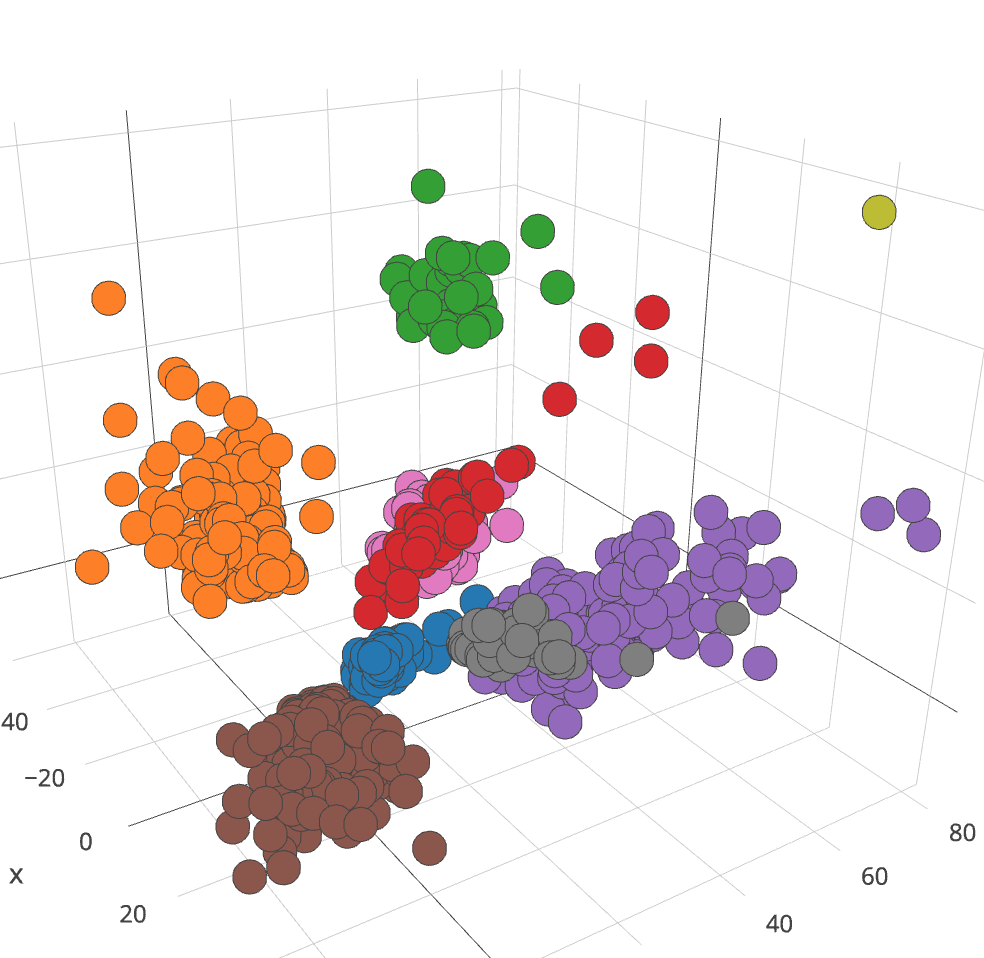
\includegraphics[width =\textwidth]{best_pred1.png}
        \caption{Best predictions}
    \end{subfigure}%
    \begin{subfigure}[b]{0.48\textwidth}
        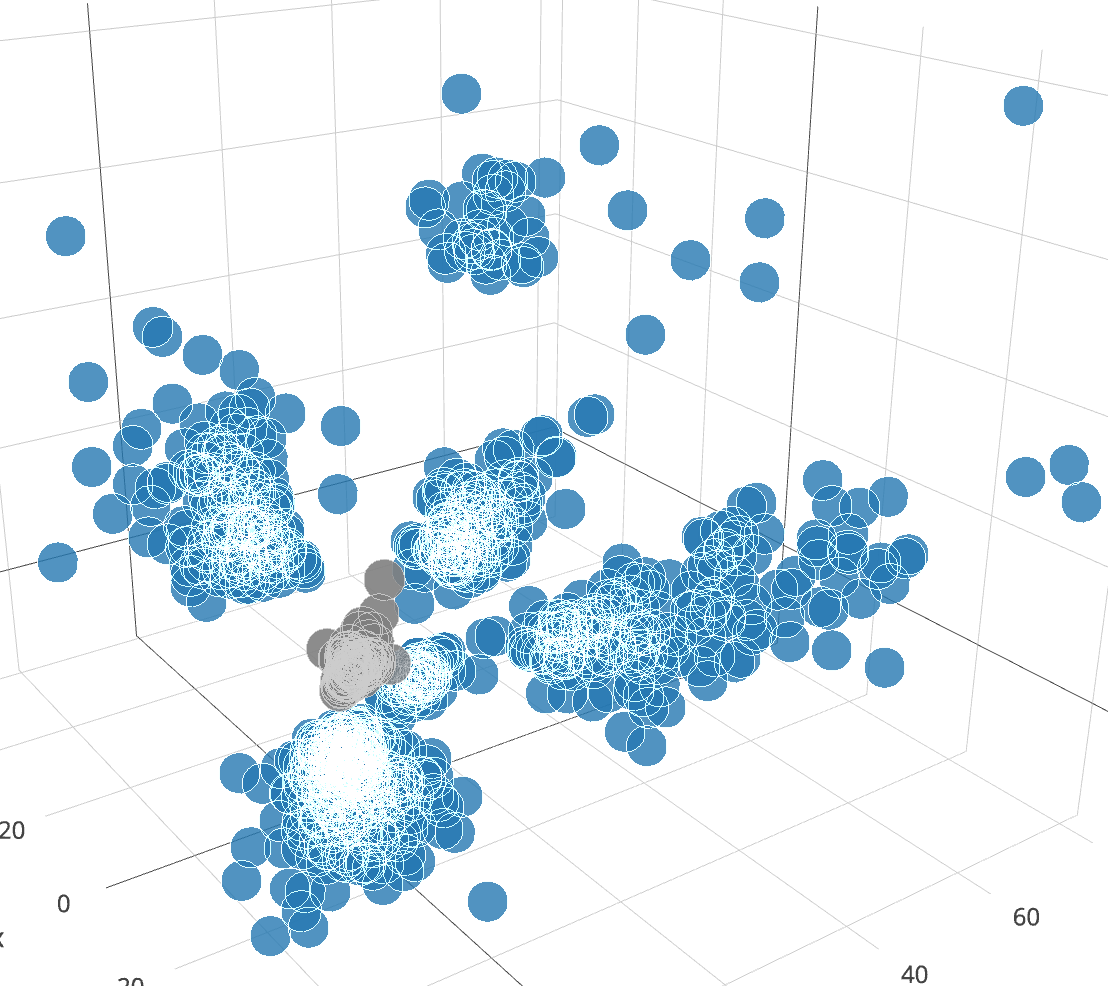
\includegraphics[width =\textwidth]{best_pred2.png}
        \caption{Best and worst predictions}
    \end{subfigure}%        
    \caption{Distribution of best and worst predictions by the model. First picture shows the location of samples that are classified well, with highest score assigned by the model. Second image shows all these samples as blue ones and some of the misclassified samples (gray).}%
    \label{fig:best_pred}%
\end{figure}

\subsubsection{Visualizations with dimensionality reduction techniques}
Even with 3-dimensional layer in class predictor, forcing the model to use such a small layer causes the decrease of its performance. To avoid this, some of the dimensionality reduction techniques may be used to obtain the representation of the data in $\mathbb{R}^{3}$. The used approach was PCA, that transforms the data by projecting them onto the directions determined by the principal vectors of the points correlation matrix. To obtain best possible approximation of the data, the vectors corresponding to the greatest principal values should be chosen. 
\par
Firstly, the correlation matrix was computed for both $F_{MNIST}$ and $F_{MNIST-M}$. Both of these point clouds are D-dimensional, so the matrices had size $D\times D$. When the singular values of the matrices were computed, the greatest 3 of them were not much greater than many others. It confirms, that the obtaining a good feature extractor demands the dimensionality of feature extractor to be much higher than $\mathbb{R}^{3}$. Therefore, projecting the data onto just 3 vectors caused a huge loss of the information. 
\par
Figure~\ref{fig:dim_red} presents the visualizations of $F_{MNIST}$ and $F_{MNIST-M}$ obtained with PCA and Kernel-PCA with RBF kernel, that firstly transforms the input data to some higher-dimensional space. The results are not as impressive as with 3-dimensional layer in the model. However, it can be clearly seen that applying GRL makes the point clouds much more similar. 

\begin{figure}[H]%
    \centering
    
    \begin{subfigure}[b]{0.33\textwidth}
        \includegraphics[width =\textwidth]{pca_nogrl.png}
        \caption{PCA, without GRL}
    \end{subfigure}%
    \begin{subfigure}[b]{0.33\textwidth}
        \includegraphics[width =\textwidth]{pca_grl.png}
        \caption{PCA, with GRL}
    \end{subfigure}%
    \begin{subfigure}[b]{0.33\textwidth}
        \includegraphics[width =\textwidth]{kpca.png}
        \caption{Kernel-PCA on $F_{MNIST}$}
    \end{subfigure}%
    \caption{The visualizations with dimensionality reduction techniques. First two pictures presents the point clouds for source (blue) and target (gray) domain, transformed to $\mathbb{R}^{3}$ with PCA method. Applying GRL during training results in more similar point clouds. The last picture presents distribution of each digit with Kernel PCA used to reduce the dimensionality.}%
    \label{fig:dim_red}%
\end{figure}

\subsubsection{Other visualizations}
The well trained feature extractor $G_{3}$ could be used to visualize the transformation made by conceptor. With MNIST as source domain and MNIST-M as target distribution, the ellipsoid approximating the $F_{MNIST}$ could be computed and represented as conceptor $C_{MNIST}$. The quota $Q(C_{MNIST})$ value was close to 1 for even small values of aperture $\alpha$. This seems reasonable, as the obtained multi-armed star cannot be captured with nothing but a sphere. Therefore, the $C_{MNIST}$ matrix was close to the identity matrix, so multiplying the samples of $F_{MNIST-M}$ by $C_{MNIST}$ did not make the point cloud more similar to $F_{MNIST}$. Figure~\ref{fig:vconc} presents the result of such transformation.
\begin{figure}[H]%
    \centering
    
    \begin{subfigure}[b]{0.27\textwidth}
        \includegraphics[width =\textwidth]{vconc1.png}
    \end{subfigure}%
    \begin{subfigure}[b]{0.27\textwidth}
        \includegraphics[width =\textwidth]{vconc2.png}
    \end{subfigure}%
    \begin{subfigure}[b]{0.27\textwidth}
        \includegraphics[width =\textwidth]{vconc3.png}
    \end{subfigure}%

    \caption{Transformation the $F_{MNIST-M}$ point cloud woth $C_{MNIST}$. First picture shows point clouds $F_{MNIST}$ (blue) and $F_{MNIST-M}$ (gray) obtained after the training (domain predictor with GRL was not used). The second picture presents the transformation of the $F_{MNIST-M}$ point cloud (gray) by conceptor $C_{MNIST}$ (green). The difference is almost imperceptible. The last picture shows all three point clouds together.}% 
    \label{fig:vconc}%
\end{figure}
\par
The multiplication by conceptor matrix only reduced the area of the point cloud. As every conceptor matrix $C$ is a positive semidefined matrix \cite{conc}, it can be presented as $C = U\Sigma U^{T}$, where $U$ and $U^{T}$ can be interpreted as rotation matrices and $\Sigma$ is a diagonal matrix with singular values of $C$ on diagonal. As all singular values of conceptor matrix are real numbers from range $[0,1]$, the conceptor matrix multiplication is in fact rotation, shortening (as non-zero values of $\Sigma$ are $\leq 1$ \cite{conc}) in certain directions and then re-rotation of the point cloud (see figure~\ref{fig:ConceptorRotation}).

\begin{figure}[H]%
    \centering
    \begin{subfigure}[b]{0.24\textwidth}
        \includegraphics[width =\textwidth]{C1.png}
        \caption{$F_{M}$}
    \end{subfigure}%
    \begin{subfigure}[b]{0.24\textwidth}
        \includegraphics[width =\textwidth]{C2.png}
        \caption{$U^{T} \cdot F_{M}$}
    \end{subfigure}%
    \begin{subfigure}[b]{0.24\textwidth}
        \includegraphics[width =\textwidth]{C3.png}
        \caption{$\Sigma \cdot U^{T} \cdot F_{M}$}
    \end{subfigure}%    
    \begin{subfigure}[b]{0.24\textwidth}
        \includegraphics[width =\textwidth]{C4.png}
        \caption{$U \cdot \Sigma \cdot U^{T} \cdot F_{M}$}
    \end{subfigure}%    
    
    \caption{$F_{MNIST}$ point cloud (denoted as $F_{M}$) transformation by its own conceptor $C_{MNIST}$. The  $F_{MNIST}$ (blue points) is firstly rotated (gray), then scaled (yellow) and finally re-rotated (green)}%
    \label{fig:ConceptorRotation}%
\end{figure}
\par
During all the experiments the activation function was \textit{leaky-ReLU}, which does not limit the data magnitude. When hyperbolic tangent \textit{tanh}, which is a mapping $\mathbb{R} \rightarrow (-1, 1)$, was applied, the model did not manage to tune its parameters properly. After the training the accuracy on source domain test set was just 78\%, while 38\% of samples from target distribution were classified well. Moreover, the distribution of the point clouds has significantly changed. $F_{MNIST}$ and $F_{MNIST-M}$ did not resemble a multi-armed star anymore. The point clouds mapped by $G_{3}$ formed  cubes, as presented on figure~\ref{fig:tanh}. The samples of each digit were aggregated in clusters scattered over the cube. However, samples from target domain were not as organized as source distribution point cloud, what explains the very poor classification result.
\noindent%
\begin{figure}[H]%
    \centering
    \begin{subfigure}[b]{0.48\textwidth}
        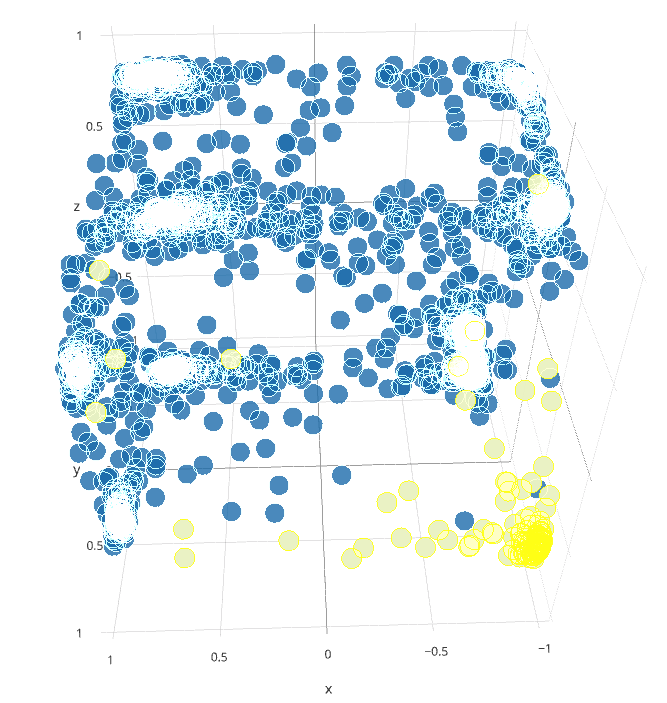
\includegraphics[width =\textwidth]{tanh1.png}
        \caption{$F_{MNIST}$}
    \end{subfigure}%
    \begin{subfigure}[b]{0.48\textwidth}
        \includegraphics[width =\textwidth]{tanh2.png}
        \caption{$F_{MNIST}$ and $F_{MNIST-M}$}
    \end{subfigure}%        
    \caption{$F_{MNIST}$ and $F_{MNIST-M}$ transformed by $G_{3}$ with \textit{tanh} as an activation function. First picture presents the distribution of $F_{MNIST}$ and zero digit images from MNIST test set (yellow). Samples from each class are grouped in clusters. The second picture shows also the location of $F_{MNIST-M}$. Target domain point cloud is unorganized, therefore the model is unable to classify it well.}%
    \label{fig:tanh}%
\end{figure}

\section{Conclusion}
During the research the gradient reversal layer was tested in many configurations and modifications. Unquestionably GRL greatly improves the model performance in domain adaptation. The different gradient modifications showed that the most important operation is inverting the gradient's sign. Applying a domain predictor with GRL to more layers of the model is a good approach that may improve the results. The hyperparameters selection, like optimization algorithm or regularization, is also a key to success.
\par
However, obtaining domain shift invariant feature vector is not possible with just GRL. The distribution information is kept in the feature vector after the training. Nonetheless, the representation that is unclear for a single domain predictor causes a significant improvement, therefore some techniques that would increase the domain invariance would definitely be valuable in domain adaptation.
\par
Usage of the conceptors in DA did not succeed within this thesis. First approach was to build a new adaptation technique based on the conceptor matrix, but it failed. Also the analysis of the high dimensional point cloud with ellipsoid described by the concpetor was rather unproductive.
\par
Including a 3-dimensional layer inside the network's architecture is a great approach to visualize the model's behaviour. The visualizations form this paper explains the domain adaptation problem and confirm the improvement when GRL is applied. Also some troubles during training the model with plugged domain predictor shows, that GRL considerably handicaps the learning process.

\printbibliography

\end{document}
